\chapter{idock: protein-ligand docking}

\section{Abstract}

The increasing availability of macromolecular structural data catalyzes the development of protein-ligand docking methods. AutoDock Vina is a competitive protein-ligand docking tool well known for its fast execution and high accuracy. Nevertheless, when docking a massive number of ligands, Vina has to be run multiple times, repeating protein parsing and grid maps building over and over again. There are tremendous requests for revising Vina to reuse precalculated data and incorporate built-in support for virtual screening. Hence we developed idock, which inherits from AutoDock Vina the accurate scoring function and the efficient optimization algorithm, and significantly improves the fundamental implementation and numerical model for even faster execution. idock achieved a speedup of 3.3 in terms of CPU time and a speedup of 7.5 in terms of elapsed time on average when benchmarked on docking 10,928 drug-like ligands. Lastly we presented a real life drug discovery problem to demonstrate the utilization of idock. idock is free and open source, available at https://GitHub.com/HongjianLi/idock.

This project was published in the \textit{Proceedings of the 2012 IEEE Symposium on Computational Intelligence in Bioinformatics and Computational Biology (CIBCB)} on 9 May 2012 \citep{1153}.

\section{Introduction}

Over recent decades, there has been a continual increase in the number of new therapeutic targets available for drug design. Advances in crystallography and nuclear magnetic resonance spectroscopy have revealed substantial structural details of proteins and protein–ligand complexes. The structures of biological macromolecules at atomic level are being routinely resolved and deposited into the world's largest and freely accessible repository called Protein Data Bank (PDB) \citep{539,537}. Meanwhile, the biological activity data of small molecules are also being regularly collected into public databases such as ChEMBL \citep{1424} and PubChem \citep{1422}. As of 15 Sep 2014, there are 103,199 structures in PDB, 1,638,394 compounds records in ChEMBL and 1,112,090 bioassays in PubChem. The rapid evolution of structure resolving techniques and the availability of structural and bioactivity resources highly catalyze the development of protein-ligand docking methods for structure-based virtual screening. Very often, the target protein is a viral enzyme of interest, and the small organic ligands that are predicted to inhibit the viral enzyme are what we want to discover.

Protein-ligand docking is a method which predicts the preferred conformation and binding affinity of a small ligand when bound to a macro protein to form a stable complex. The ligand conformation refers to its spatial position, orientation, and torsions, if any. Figure \ref{idock:MRV} shows the crystal conformation and a docked conformation of the marketed HIV drug maraviroc in complex with the human CCR5 chemokine receptor (PDB: 4MBS). The protein is rendered in molecular surface representation, where positively- and negative-charged regions are in blue and red, respectively. The ligand is rendered in stick representation with the same color scheme, where oxygen and nitrogen atoms are in blue and red, respectively. The binding cavity on the protein surface is depicted by a green cubic box. The putative intermolecular hydrogen bonds are shown as cyan dashed lines. The docked conformation was predicted by idock \citep{1153} and the figure was rendered by iview \citep{1366}.

\begin{figure}
\centering
\subfloat[Crystal conformation.]
{
  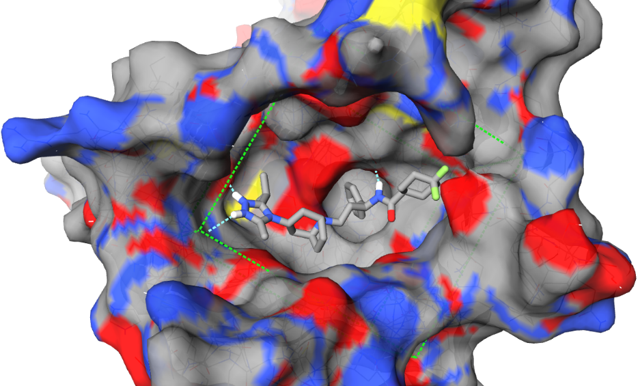
\includegraphics[width=0.48\linewidth]{../usrt/MRV0.png}
}
\subfloat[Docked conformation.]
{
  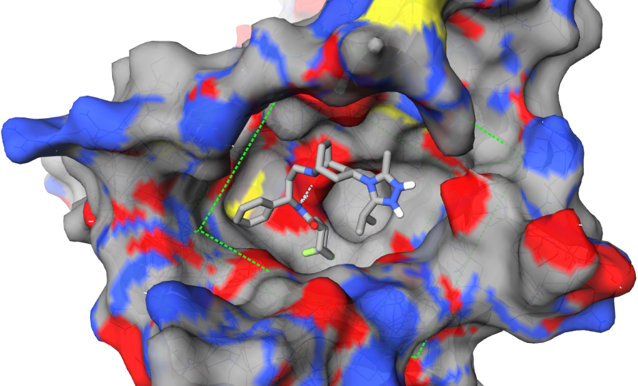
\includegraphics[width=0.48\linewidth]{../usrt/MRV1.png}
}
\caption{An intuitive example of two conformations of a ligand. }
\label{idock:MRV}
\end{figure}

The binding affinity is a numerical value that suggests how strongly the interactions are formed between the protein and the ligand upon binding. Empirically, it is the overall effect of various chemical interactions involved, such as van der Waals force, electrostatic force, salt bridges, hydrogen bonding, hydrophobic effects, pi interactions, halogen interactions, metal interactions, and the like. It is usually estimated by the scoring function employed in a docking tool. The binding affinity is usually expressed in pKd unit, which is the negative logarithm of dissociation constant Kd. In Figure \ref{idock:MRV} the binding affinities of the crystal and docked conformations were predicted to be 8.27 and 8.01 pKd, respectively, by RF-Score \citep{564}. The binding affinity can be alternatively expressed in terms of free energy $\Delta G$ in kcal/mol unit, which is usually a negative value. The lower the free energy, the higher the binding affinity.

Structure-based virtual screening can be regarded as a massive version of docking. Instead of a single ligand, a database of ligands are docked against the target protein, then ranked according to their predicted binding affinity, and finally the top ones are selected for further investigations.

When a docking program is treated as a black box, its input includes the 3D structures of a protein and a ligand, and its output includes several predicted conformations and their predicted binding affinity. Regarding the protein input, the PDB database \citep{539,537} almost serves as the unique \textit{de facto} data source. Regarding the ligand input, there are dozens of data sources. The GDB-17 database \citep{1276} enumerates 166 billion organic small molecules. The PubChem database \citep{526} comprises 53 million unique structures. The ZINC database \citep{532,1178} contains over 35 million purchasable compounds in ready-to-dock, 3D formats. The TCM@Taiwan database \citep{528} comprises 37,170 TCM (Traditional Chinese Medicine) compounds from 352 TCM ingredients. Regarding the output visualization and analysis, PyMOL \citep{1221}, Chimera \citep{1219}, VMD \citep{1220}, AutoDockTools4 \citep{596}, ViewDock TDW \citep{559}, PoseView \citep{748} and LigPlot+ \citep{951} are popular tools to visualize docked conformations and plot putative interaction charts. AuPosSOM \citep{598} can be used to cluster docked conformations. BEDROC \citep{490} and SLR \citep{489} can be used as statistical metrics for docking method evaluation.

When a docking program is treated as a white box, it consists of two typical components, an algorithm to explore the conformational space, and a scoring function to predict the binding affinity given a sampled conformation. There is a huge body of docking tools, e.g. DOCK \citep{1222,1445}, AutoDock 4 \citep{596}, AutoDock Vina \citep{595}, QuickVina \citep{1193}, PLANTS \citep{610,607,779}, FITTED \citep{602,603}, CDOCK \citep{1224}, CRDOCK \citep{1200}, and PharmDock \citep{1376}, as well as scoring functions, e.g. RF-Score \citep{564,1370}, SFCscore \citep{581,1347}, LISA \citep{775}, and NNScore 2.0 \citep{977}. More can be found in survey papers \citep{493,922}.

Amongst a sea of docking programs, AutoDock Vina \citep{595} (hereafter Vina for short) is a competitive one because not only it is free and open source under Apache License 2.0, but also it has been shown to improve the average accuracy of the binding mode predictions \citep{595} and run faster than its predecessor AutoDock 4 \citep{596} by an order of magnitude when benchmarking on virtual screening for HIV protease inhibitors \citep{556}. Released in the second half of 2010, Vina has been cited over 1,000 times and adopted by a wide community of researchers. Apart from the Vina docking tool itself, there is a PyMOL plugin for AutoDock and Vina \citep{609}. MOLA \citep{773} is a bootable, self-configuring system for virtual screening using AutoDock4/Vina on computer clusters. VSDK \citep{1268} is a console application system of virtual screening of small molecules using AutoDock Vina on Windows. AUDocker LE \citep{1250} is a GUI for virtual screening with AutoDock Vina on Windows. All these auxiliary tools facilitate the use of Vina under various settings.%TODO: update Vina citation count.

Vina is attractive thanks to a series of success stories by third parties. To name a few, Vina was used for 1) docking studies on the HEPT derivatives of HIV-1 reverse transcriptase \citep{843}, 2) for side-chain residue flexibility study of VEGFR-2 (Vascular Endothelial Growth Factor Receptor 2), which is a known protein target for anti-angiogenic agents \citep{1084}, 3) for identification of novel inhibitors of sirtuin 2, which is a NAD\textsuperscript{+}-dependent histone deacetylase enzyme \citep{1177}, and 4) for repurposing study of FDA-approved drugs for cancer therapy in order to screen for compounds that potentially inhibit MDM2, which an E3 ubiquitin ligase that polyubiquitinates p53 \citep{1230}. Such exciting success stories prove the real power of protein-ligand docking, Vina in particular, for computer-aided drug discovery.

Although Vina is popular and competitive and well known for its fast execution and high accuracy, it is optimized for single-ligand docking rather than virtual screening. When it comes to docking a large pool of ligands, Vina has to be invoked multiple times, repeatedly parsing the same protein and creating the same internal data structures such as grid maps. There are enormous requests from the community for modifying and recompiling Vina to make it support virtual screening in a superfast manner by reusing protein data and grid maps. We were motivated by the desire to provide built-in support for virtual screening and therefore developed idock. Moreover, we incorporated quite many implementation tricks to further speedup idock. Lastly, we utilized idock to attempt to address a real life drug discovery problem.

\section{Methods}

\subsection{Flowchart}

Figure \ref{idock:Flowchart} shows the overall flowchart of idock. During initialization, idock precalculates the scoring function for all possible combinations of atom type pairs and interatomic distances. It parses the protein and determines the atom types with the help of residue sequence, and creates a thread pool to hold reusable threads. Then it enters a loop and fetches a ligand from a user-specified input folder to perform docking. It parses the ligand and determines the atom types with the aid of branch information, and meanwhile automatically detects and deactivates inactive torsions. It builds grid maps of granularity 0.15625 \AA\ by default on the fly with multithreading, and distributes multiple independent Monte Carlo tasks to the thread pool for concurrent execution. Then it merges the conformations from separate threads and clusters them with RMSD 2.0 \AA, and writes them to the user-specified output folder and displays the predicted free energy on screen. It automatically proceeds with the next ligand until all are docked. Finally it destroys the thread pool and releases memory resources.

\begin{figure}
\centering
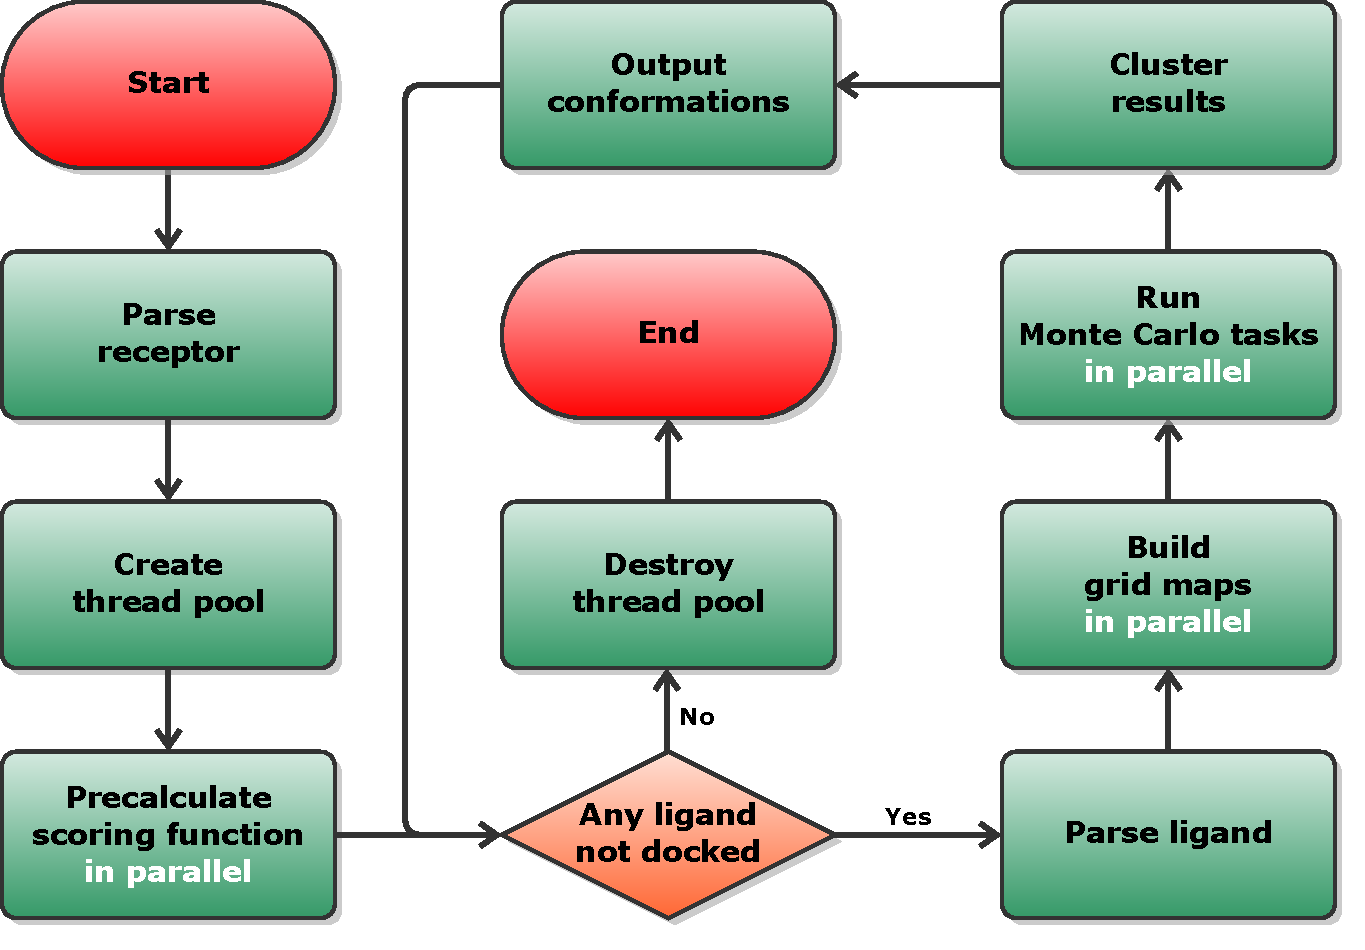
\includegraphics[width=\linewidth]{../idock/Flowchart.pdf}
\caption{idock flowchart.}
\label{idock:Flowchart}
\end{figure}

\subsection{PDBQT specification}

PDBQT is the protein and ligand input and output format used by AutoDock \citep{597,596}, Vina \citep{595}, idock \citep{1153}, and QuickVina \citep{1193}. Its official definition is at http://autodock.scripps.edu/faqs-help/faq/what-is-the-format-of-a-pdbqt-file. In PDBQT format (Figure \ref{idock:PDBQT}), ligands can be treated as flexible with the idea of a torsion tree to represent the rigid and rotatable pieces. There is always one root, and zero or more branches. Branches can be nested. Every branch defines a rotatable bond.

\begin{figure}
\centering
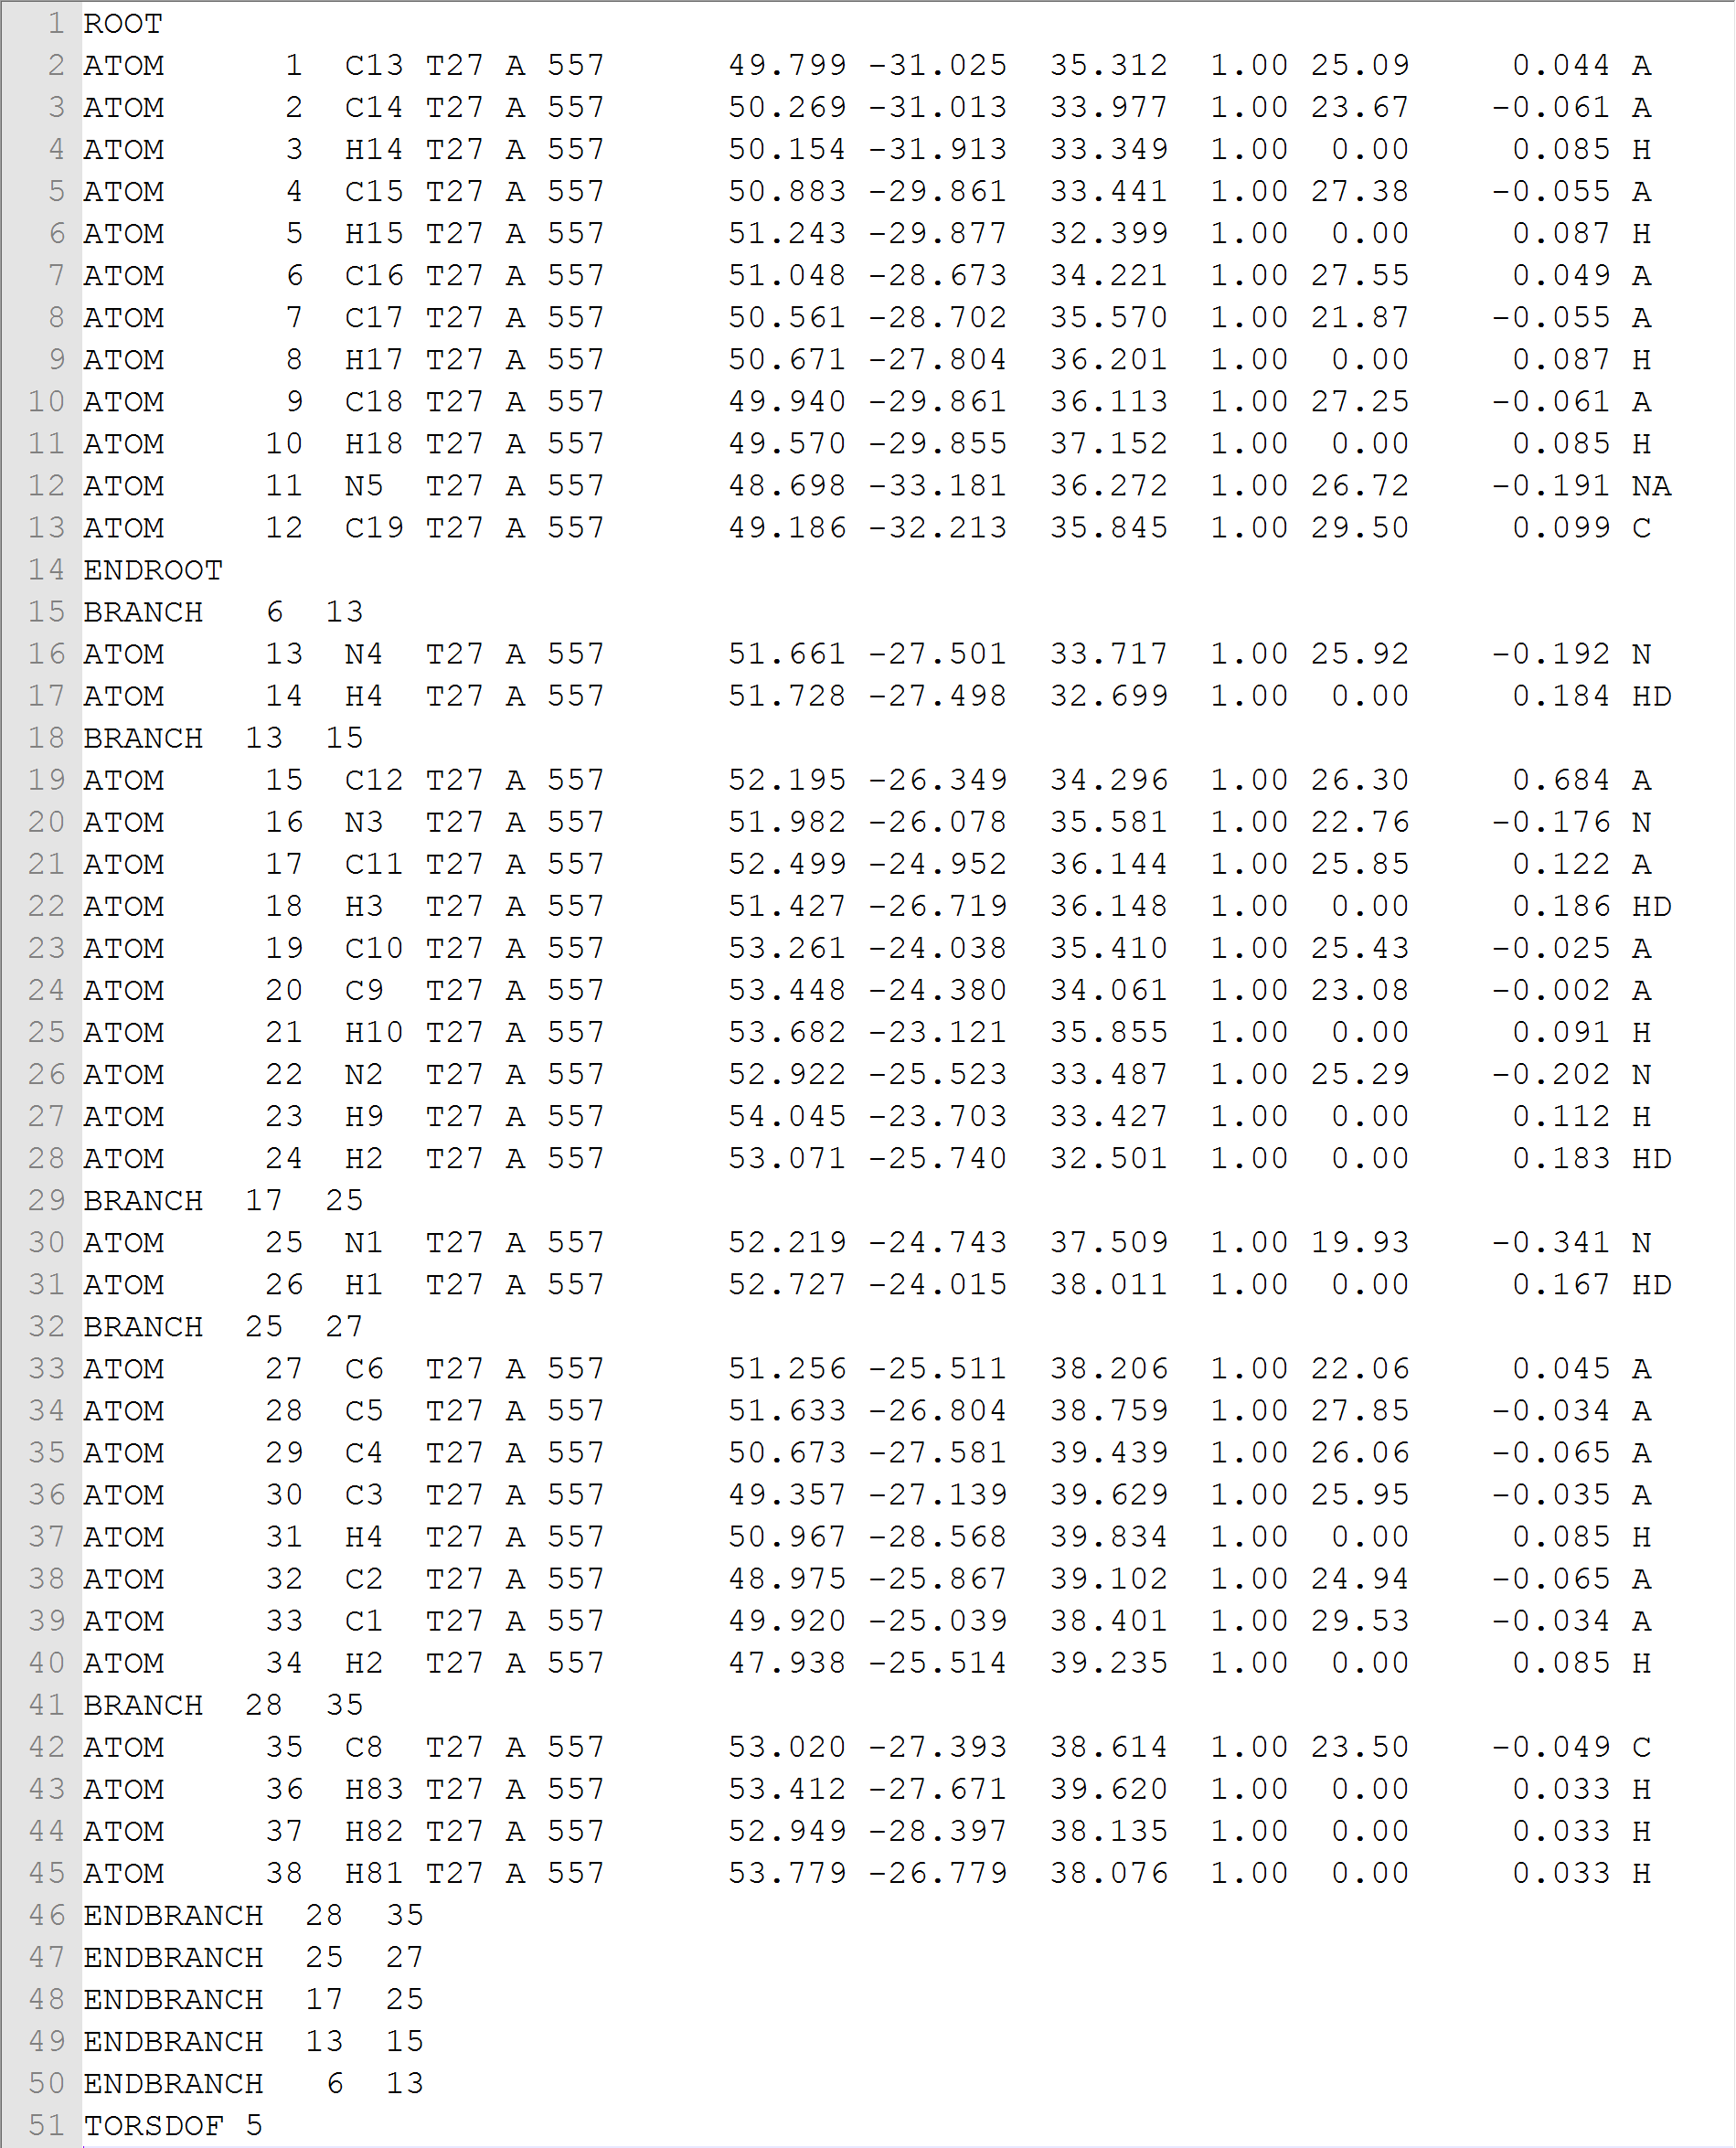
\includegraphics[width=\linewidth]{../usrt/T27CrystalPDBQT.png}
\caption{PDBQT content of a ligand.}
\label{idock:PDBQT}
\end{figure}

The torsion tree is represented with some records specific to the PDBQT format. A ROOT record precedes the rigid part of the molecule, from which zero or more rotatable bonds may emanate. The rigid root contains one or more ATOM or HETATM records in PDBQT style. These records resemble their traditional PDB counterparts, but diverge in columns 71-79 inclusive, where the first character in the line corresponds to column 1. The Gasteiger partial charge is stored in columns 71-76 inclusive in \%6.3f format, i.e. right-justified, 6 characters wide, with 3 decimal places. The AutoDock atom-type is stored in columns 78-79 inclusive in \%-2.2s format, i.e. left-justified and 2 characters wide. An ENDROOT record follows the last atom in the rigid root. The ROOT/ENDROOT block of atoms is given first in the PDBQT file.

Sets of atoms moved by rotatable bonds are enclosed by BRANCH and ENDBRANCH records. These BRANCH/ENDBRANCH blocks follow the ROOT/ENDROOT block. Both BRANCH and ENDBRANCH records give two integers specifying the serial numbers of the first and second atoms involved in the rotatable bond. BRANCH/ENDBRANCH blocks can be nested. The last atom in a branch is followed by an ENDBRANCH record, whose serial numbers of the two atoms in the rotatable bond match those in the corresponding BRANCH record.

The last line contains a TORSDOF record, which is followed by an integer specifying the number of torsional degrees of freedom in the ligand.

\subsection{Conformational modeling}

A conformation refers to a combination of position, orientation, and torsions, if any. Figure \ref{idock:DOF} shows the positional, orientational and torsional degree of freedom. In (a), the two conformations in different colors only differ in their spatial position. One conformation can be transformed to the other simply by a spatial translation. In (b), the two conformations only differ in their orientation. One conformation can be transformed to the other simply by a spatial rotation. In (c), the two conformations only differ by one torsion. One conformation can be transformed to the other by a rotation along the rotatable bond, shown in the center of the subfigure, by a certain degree applied only to the child branches of that rotatable bond.

\begin{figure}
\centering
\subfloat[Positional degree of freedom.]
{
  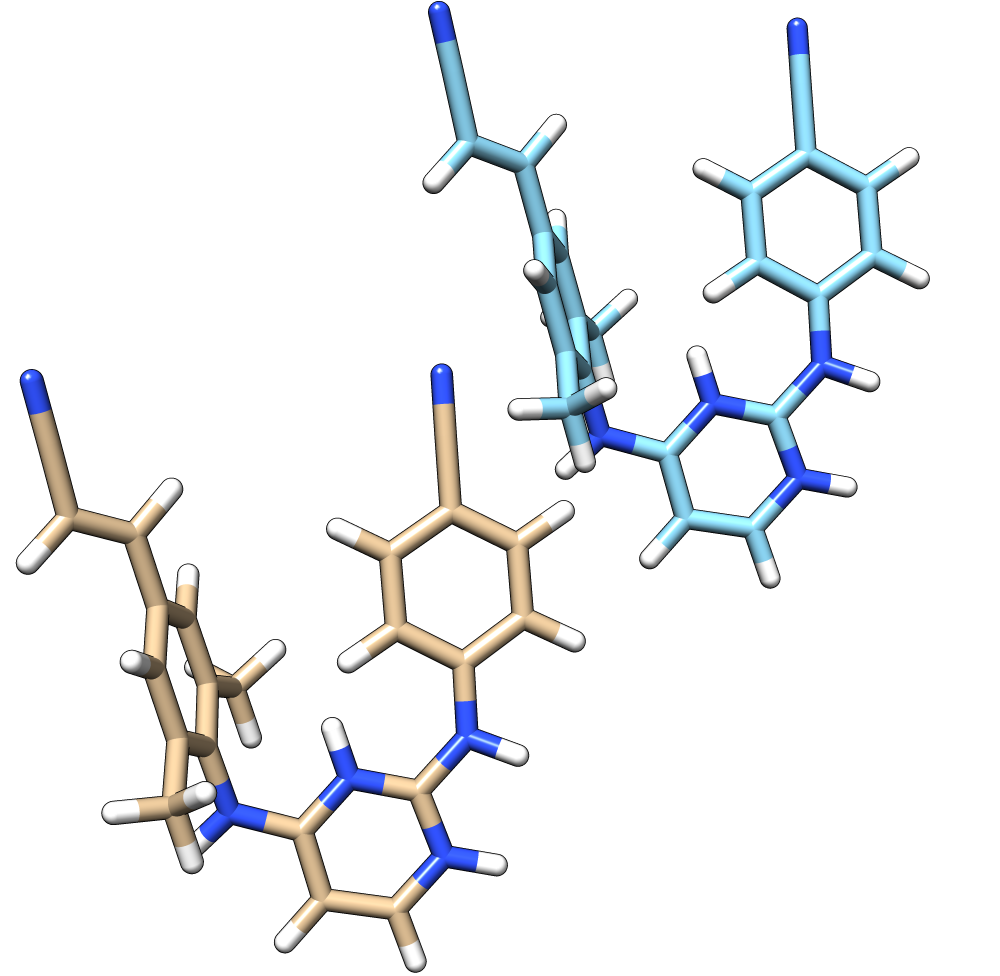
\includegraphics[width=0.32\linewidth]{../idock/PositionalDOF.png}
}
\subfloat[Orientational degree of freedom.]
{
  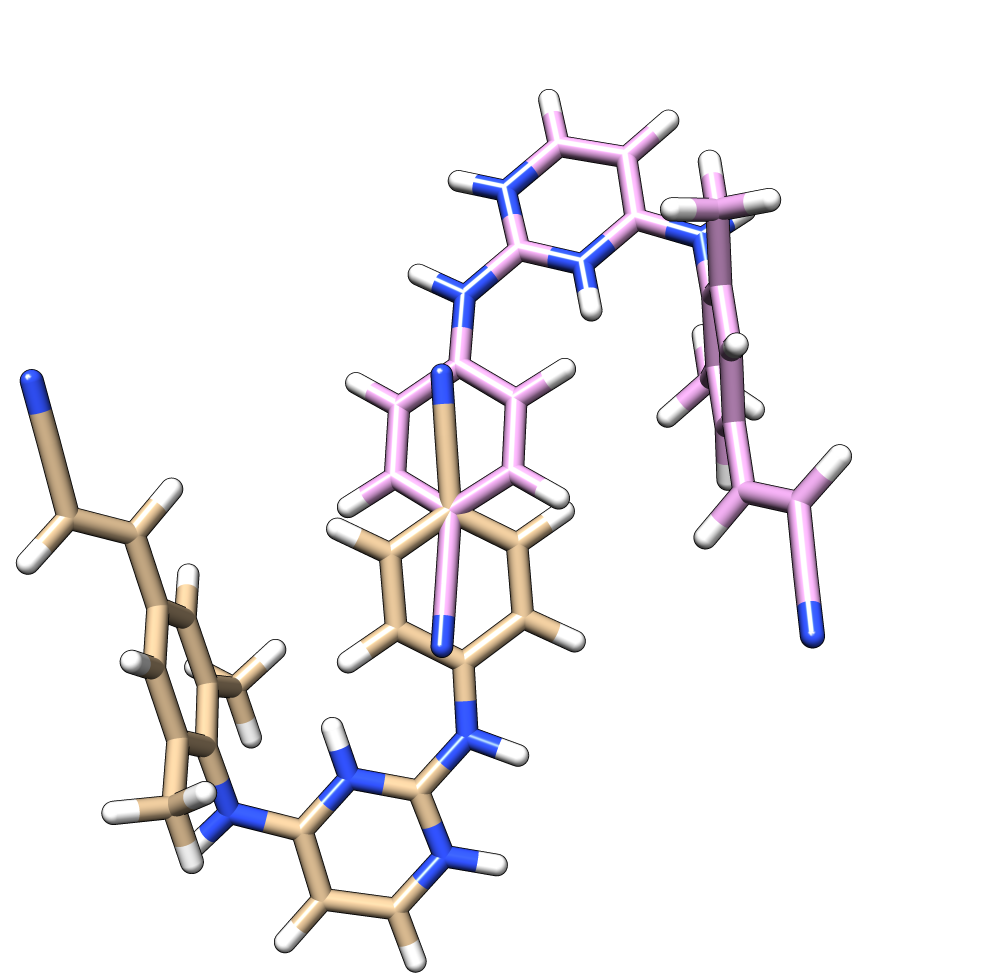
\includegraphics[width=0.32\linewidth]{../idock/OrientationalDOF.png}
}
\subfloat[Torsional degree of freedom.]
{
  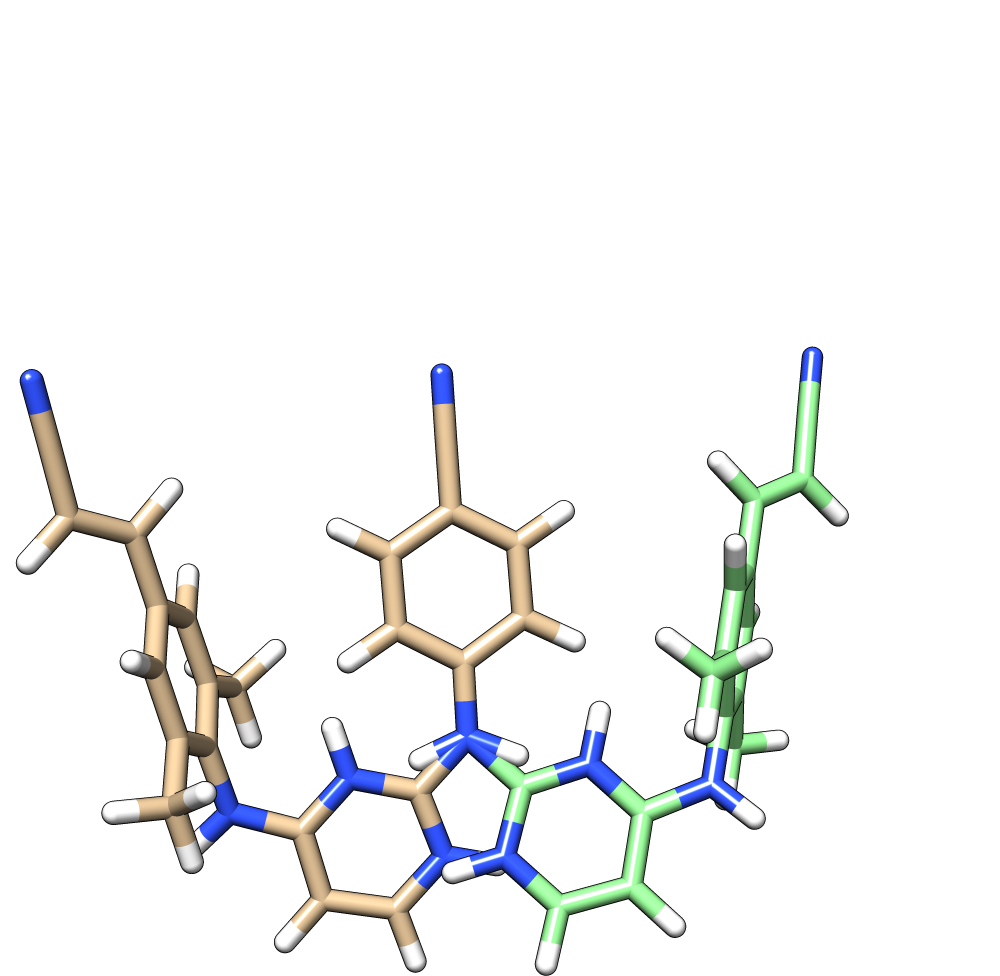
\includegraphics[width=0.32\linewidth]{../idock/TorsionalDOF.png}
}
\caption{Conformational degree of freedom.}
\label{idock:DOF}
\end{figure}

In the root or any branch, the atomic positions are relative to each atom because of no rotatable bond therein. Hence it is possible to model the conformation of the root or a branch by the the 3D coordinate of a reference atom as well as a normal vector to represent the orientation, while the positions of the other atoms in the same branch can be recovered with the relative atomic positions. The reference atom can be chosen to be the atom connecting the parent branch, i.e. the second atom involved in the rotatable bond or the Y atom in the line of ``BRANCH X Y". It is always the first atom of the current branch if the PDBQT file is produced by AutoDockTools4 \citep{596}. As for the representation of orientation, a normalized quaternion typically features better numerical stability than a directional triplet.

Once the conformation of the root or a branch is determined, the orientation of a child branch can be derived by that of the parent branch and a torsion, which is essentially the rotating angle along the connecting rotatable bond and is thus in the range of $[–\pi, \pi]$. The position of the reference atom of the child branch (the Y atom) is fixed relative to the first atom involved in the connecting rotatable bond (the X atom) and is invariant of the torsion applied. Therefore, the conformation of a child branch can be uniquely identified by the conformation of its parent branch and a torsion value. Eventually in a cascade way, the conformation of a flexible ligand can be modeled by the conformation of the root and a set of torsion values as many as the number of rotatable bonds.

Mathematically, a ligand conformation can be modeled by a numerical vector $\mathbf c=(x, y, z, q_0, q_1, q_2, q_3, t_1, t_2, ..., t_n)$, where $(x, y, z)$ represents the position of the reference atom (the first atom) of the root, $(q_0, q_1, q_2, q_3)$ represents the orientation of the root, with $q_0^2+q_1^2+q_2^2+q_3^2=1$, and $(t_1, t_2, ..., t_n)$ represents the torsions of all child branches, with $n$ being the number of rotatable bonds and $t_i\in[-\pi, \pi]$ for $i\in[1, n]$. The conformational degree of freedom is at least 6, 3 from the position and 3 from the orientation. Nowadays modern drugs usually have 4 or more torsions, so the conformational degree of freedom is generally at least 10.

\subsection{Scoring function}

The scoring function estimates the binding affinity given a conformation (equation \eqref{idock:f}). The binding affinity is expressed in terms of free energy. The lower the free energy, the higher the binding affinity.

\begin{equation}
\label{idock:f}
e = f(\mathbf c) = f(x, y, z, q_0, q_1, q_2, q_3, t_1, t_2, ..., t_n)
\end{equation}

Both idock and Vina share the same scoring function, which consists of a conformation-dependent part and a conformation-independent part. The conformation-dependent part is a weighted sum of five terms over all the pairs of atom $i$ and atom $j$ that can move relative to each other. It is calculated from equations \eqref{idock:e} and \eqref{idock:e_ij} where $t_i$ and $t_j$ are the atom types of $i$ and $j$ respectively, and $r_{ij}$ is their interatomic distance. The five terms are calculated from equations \eqref{idock:Gauss1} to \eqref{idock:HBonding} where $d_{ij}$ is the surface distance calculated from equation \eqref{idock:d_ij} where $R_{t_i}$ and $R_{t_j}$ are the Van der Waals radii of $t_i$ and $t_j$ respectively (Figure \ref{idock:Distance}). All the units are in \AA. The weighting coefficients and the cut off at $r_{ij}$ = 8 \AA\ of the five terms are borrowed from Vina. The optimization algorithm tries to find the global minimum of $e$ and other low-scoring conformations, which it ranks subsequently.

\begin{equation}
\label{idock:e}
e = \sum_{i < j} e_{ij}
\end{equation}

\begin{eqnarray}
\label{idock:e_ij}
e_{ij} &=& (-0.035579) * Gauss_1(t_i, t_j, r_{ij}) \nonumber \\
       &+& (-0.005156) * Gauss_2(t_i, t_j, r_{ij}) \nonumber \\
       &+& (+0.840245) * Repulsion(t_i, t_j, r_{ij}) \nonumber \\
       &+& (-0.035069) * Hydrophobic(t_i, t_j, r_{ij}) \nonumber \\
       &+& (-0.587439) * HBonding(t_i, t_j, r_{ij})
\end{eqnarray}

\begin{equation}
\label{idock:Gauss1}
Gauss_1(t_i, t_j, r_{ij}) = e^{-(d_{ij} / 0.5)^2}
\end{equation}

\begin{equation}
\label{idock:Gauss2}
Gauss_2(t_i, t_j, r_{ij}) = e^{-((d_{ij} - 3) / 2)^2}
\end{equation}

\begin{equation}
\label{idock:Repulsion}
Repulsion(t_i, t_j, r_{ij}) =
\begin{cases}
d_{ij}^2 & \text{if } d_{ij} < 0\\
0 &\text{if } d_{ij} \geq 0
\end{cases}
\end{equation}

\begin{equation}
\label{idock:Hydrophobic}
Hydrophobic(t_i, t_j, r_{ij}) =
\begin{cases}
1 & \text{if } d_{ij} \leq 0.5\\
1.5 - d_{ij} & \text{if } 0.5 < d_{ij} < 1.5\\
0 & \text{if } d_{ij} \geq 1.5\\
\end{cases}
\end{equation}

\begin{equation}
\label{idock:HBonding}
HBonding(t_i, t_j, r_{ij}) =
\begin{cases}
1 & \text{if } d_{ij} \leq -0.7\\
d_{ij} / (-0.7) & \text{if } -0.7 < d_{ij} < 0\\
0 & \text{if } d_{ij} \geq 0\\
\end{cases}
\end{equation}

\begin{equation}
\label{idock:d_ij}
d_{ij} = r_{ij} - (R_{t_i} + R_{t_j})
\end{equation}

\begin{figure}
\centering
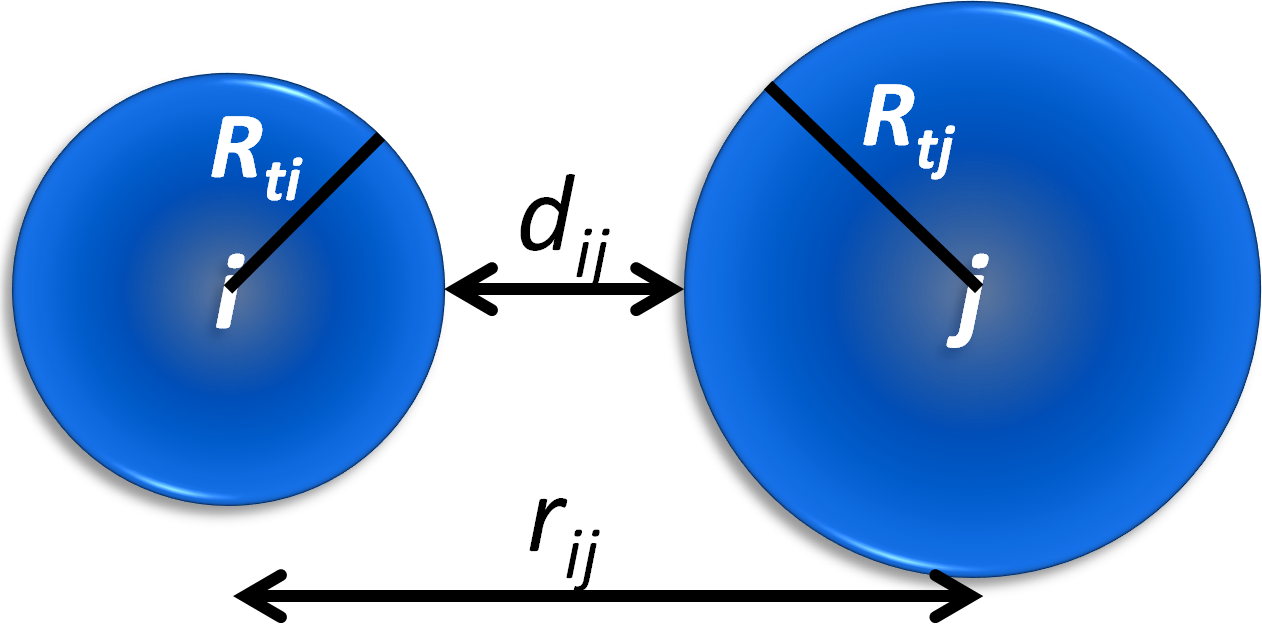
\includegraphics[width=\linewidth]{../idock/Distance.png}
\caption{Relationship between surface distance $d_{ij}$ and interatomic distance $r_{ij}$.}
\label{idock:Distance}
\end{figure}

The conformation-dependent part can be seen as the sum of intermolecular and intramolecular contributions. Hence equation \eqref{idock:e} can be rewritten into equation \eqref{idock:inter+intra} where $e_{inter}$ is the summation over all the heavy atoms between the protein and the ligand, and $e_{intra}$ is the summation over all the 1-4 ligand heavy atoms that are separated by at most three consecutive covalent bonds and can move relative to each other.

\begin{equation}
\label{idock:inter+intra}
e = e_{inter} + e_{intra}
\end{equation}

The conformation-independent part penalizes $e_{inter}$ for ligand flexibility. The predicted free energy of the $k$th conformation for output, denoted as $e'_k$, is calculated from equation \eqref{idock:FlexibilityPenalty} where $k$ is the subscript for conformation, $e_k$ is the conformation-dependent score of the $k$th conformation calculated from equation \eqref{idock:e}, $e_{intra,1}$ is the $e_{intra}$ of the first, i.e. lowest-scoring conformation, $N_{ActTors}$ is the number of active torsions and $N_{InactTors}$ is the number of inactive torsions of the ligand. Note that $e_{intra,1}$, rather than $e_{intra,k}$, acts as subtrahend in order to preserve the ranking.

\begin{equation}
\label{idock:FlexibilityPenalty}
e'_k = \frac{e_k - e_{intra,1}}{1 + 0.05846 * (N_{ActTors} + 0.5 * N_{InactTors})}
\end{equation}

The value of $e_{ij}$ is basically a function of three variables, namely $t_i$, $t_j$, and $r_{ij}$. These three variables have both a known lower bound and a known upper bound, so it is possible to precalculate the scoring function. Since there are 15 atom types implemented in idock, the pair of $t_i$ and $t_j$ can have 120 (=15*16/2) different combinations. Since $r_{ij}$ is cut off at 8 \AA, idock uniformly samples 16,384 points in range [0, 8] to turn the continuous domain into a concrete domain, resulting in an average absolute error of merely 0.002 kcal/mol. During program initialization, idock precalculates $e_{ij}$ from equation \eqref{idock:e_ij} for 120*16,384 possible combinations of $t_i$, $t_j$, and $r_{ij}$. During optimization, idock approximates the true value of $e_{ij}$ by direct assignment rather than linear interpolation so as to fast evaluate $e_{ij}$ at the cost of a little bit longer precalculation time and a bit more memory storage.

\subsection{Grid maps}

Grid maps are often built in order to fast evaluate $e_{inter}$. A grid map of atom type \textit{t} is constructed by placing virtual probe atoms of atom type \textit{t} along the X, Y, Z dimensions of the search box at a certain granularity. Figure \ref{idock:GridMap} illustrates an a grid map, where the virtual probe atoms are shown in purple. The $e_{inter}$ value of these probe atoms are precalculated, so the $e_{inter}$ value of a ligand heavy atom can be approximated in some way. In Vina, the grid map granularity is hard coded to be 0.375 \AA, and the approximation is done by linear interpolation of the 8 corner probe atoms of the residing subbox. This kind of interpolation involves reading of 8 $e_{inter}$ values, computation of 3 $\alpha$ values, 12 floating-point subtractions, 24 floating-point multiplications, and 7 floating-point additions, which turned out to be a performance bottleneck when we profiled Vina. In contrast, idock exposes grid map granularity as an optional program argument with a tuned default value of 0.15625 \AA. Likewise, due to a higher density of probe atoms, idock substitutes direct assignment for linear interpolation for much faster evaluation of $e_{inter}$ at the cost of longer precalculation time and larger memory storage. Therefore, the creation of grid maps is carried out on the fly only when necessary and abstracted into parallel tasks, which are then distributed to the thread pool for concurrent execution.

\begin{figure}
\centering
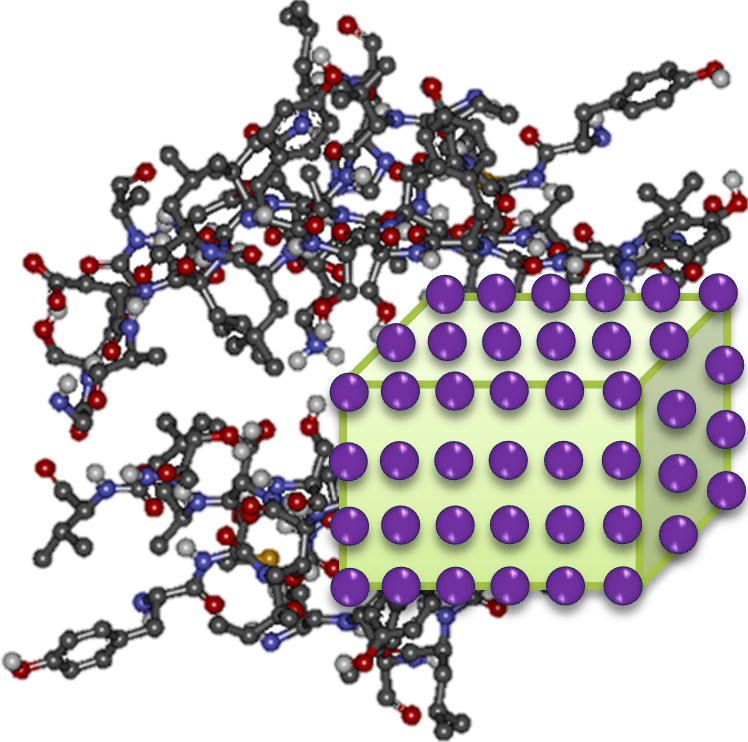
\includegraphics[width=\linewidth]{../idock/GridMap.png}
\caption{Grid map for fast evaluation of $e_{inter}$}
\label{idock:GridMap}
\end{figure}

\subsection{Optimization algorithm}

Both idock and Vina use Monte Carlo algorithm for global optimization and Broyden-Fletcher-Goldfarb-Shanno (BFGS) \citep{786} Quasi-Newton method for local optimization. Figure \ref{idock:MonteCarlo}, modified from the Figure 2 in \citep{493}, shows this optimization procedure. A succession of steps consisting of a mutation and a BFGS local optimization are taken, with each step being accepted according to the Metropolis criterion. These steps are repeated over \textit{N} iterations, where \textit{N} correlates to the complexity of the ligand regarding number of heavy atoms and number of torsions. BFGS approximates the inverse Hessian matrix of the scoring function. It uses not only the value of the scoring function but also its gradient, which are the derivatives of the scoring function with respect to the position and orientation of the ligand, and the torsions for the active rotatable bonds in the ligand. A BFGS iteration derives a descent direction from the approximate inverse Hessian matrix, derives a step length along the descent direction by line search, and updates the approximation of inverse Hessian matrix. Both programs achieve multithreading by concurrently running multiple independent Monte Carlo tasks starting from random initial conformations.

\begin{figure}
\centering
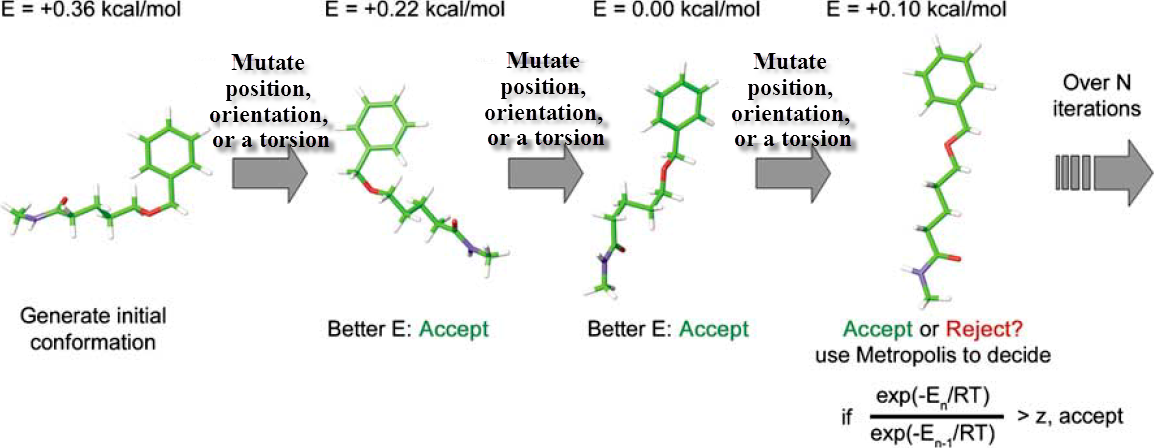
\includegraphics[width=\linewidth]{../idock/MonteCarlo.png}
\caption{Monte Carlo optimization algorithm.}
\label{idock:MonteCarlo}
\end{figure}

Though both programs share similar optimization algorithms, their implementations differ. Compared with Vina, the Monte Carlo iterations in idock are far fewer and the BFGS iterations are more. On one hand, the fewer number of Monte Carlo iterations is compensated by a larger number of parallel Monte Carlo tasks, which is 64 by default in idock compared to 8 in Vina, guaranteeing better conformational diversity and higher CPU utilization on multi-core computers. On the other hand, the stopping criterion of BFGS local optimization does not depend on an estimated number of iterations, which is the case in Vina, but depends on the outcome of line search. The BFGS local optimization stops if and only if no appropriate step length can be obtained by line search, thus increasing the probability of finding optimal local minimums.

\subsection{Native support of virtual screening}

Vina is optimized for single-ligand docking rather than virtual screening. When it comes to docking a large pool of ligands, Vina has to be invoked multiple times, repeatedly parsing the same protein and creating the same grid maps, thus degrading performance.

idock supports virtual screening in a native manner. It docks a directory of ligands instead of a single ligand, and reuses protein and grid maps (note the loop in the flowchart in Figure \ref{idock:Flowchart}). Given a very large amount of ligands to dock, idock indirectly supports two-phase virtual screening via two consecutive runs. In the first run, idock performs coarse but fast virtual screening without writing any conformations to file, aiming to quickly shortlist a few candidate compounds. This can be done by setting the grid map granularity to a coarse value and setting the maximum number of output conformations to zero. In the second run, idock performs fine but slow virtual screening with a significantly larger number of Monte Carlo tasks per ligand, writing as many conformations to file as possible and aiming to refine the predicted free energy as well as predicted conformation of candidate compounds. Such a 2-phase docking methodology can remarkably reduce overall execution time while avoiding the risk of filtering out potentially promising compounds, controlling the false negative rate at an acceptable level.

\subsection{Detection of inactive torsions}

idock automatically detects and deactivates inactive torsions, which are presented and activated in the input file in PDBQT format but have no impact on the overall scoring, such as \textemdash{OH} and \textemdash{NH$_2$}, because they only rotate the hydrogens. Figure \ref{idock:InactiveTorsions} shows an example ligand which contains 4 active torsions defined by the python script \textit{prepare\_ligand4.py} provided by AutoDock Tools \citep{596}. Two of them, highlighted in yellow, only rotate hydrogens and thus have no contributions to the scoring. They are re-classified as inactive torsions and deactivated while being parsed in idock. This kind of automatic detection and deactivation of inactive torsions reduces the torsional degrees of freedom to optimize in the local optimization step, leading to easier finding of local minimums.

\begin{figure}
\centering
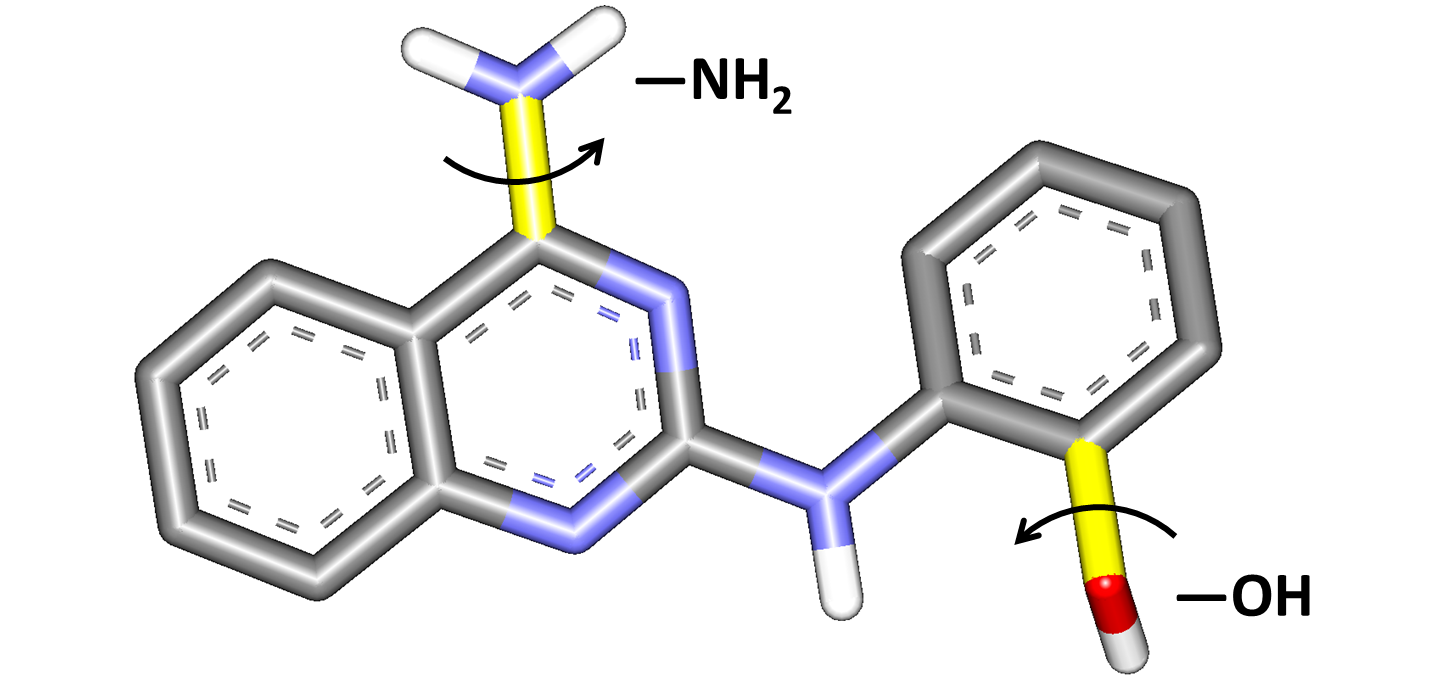
\includegraphics[width=\linewidth]{../idock/InactiveTorsions.png}
\caption{Example of inactive torsions, highlighted in yellow.}
\label{idock:InactiveTorsions}
\end{figure}

\subsection{Implementation tricks}

idock implements a lightweight thread pool in order to reuse threads and maintain a high CPU utilization throughout the entire screening procedure. During program initialization, idock creates a thread pool of $N$ threads, where $N$ is the number of CPU cores automatically detected, or can be specified by user via a command line argument. When idle, the threads sleep. When tasks arrive, the threads compete for tasks. The thread that completes its current task will automatically fetch a pending one to execute until all are done. Synchronization is implemented to ensure the full completeness of tasks and availability of results. The task here is an abstract concept in programming sense and can be instantiated either as scoring function tasks, grid map tasks or Monte Carlo tasks. To be exact, the thread pool in fact parallelizes the precalculation of scoring function, the creation of grid maps, and the execution of Monte Carlo tasks.

idock implements our own lightweight thread-safe progress bar, reporting progress every 10\% Monte Carlo tasks per ligand. idock better supports rvalue references and move semantics in C++11 to boost performance. idock flattens the tree-like recursive data structure of ligand as used in AutoDock Vina into simple linear array structure to ensure a high data cache hit rate and easy coding. idock accelerates the assignment of atom types by making use of residue information for the protein and branch information for the ligand.

idock supports reading and writing compressed ligand files with in gzip/bzip2 format, resulting in a file footprint as low as just one eighth of the raw size using gzip. This new functionality turns out to be extremely handy given an enormous amount of ligands to dock.

Both idock and Vina support 16 common chemical elements, which are H (hydrogen), C (carbon), N (nitrogen), O (oxygen), F (fluorine), Mg (magnesium), P (phosphorus), S (sulfur), Cl (chlorine), Ca (calcium), Mn (manganese), Fe (iron), Zn (zinc), Se (selenium), Br (bromine), and I (iodine). idock adds 9 additional elements, which are Na (sodium), K (potassium), Co (cobalt), Ni (nickel), Cu (copper), Sr (strontium), Cd (cadmium), Hg (mercury), and As (arsenic). Hence idock supports as many as 25 chemical elements, covering the majority of ligand atom types.

idock outputs verbose information to docked PDBQT files, including total free energy normalized by torsional degree of freedom, total free energy, inter-ligand free energy, intra-ligand free energy, putative hydrogen bonds, and per-atom inter-ligand free energy. The normalized total free energy is used in ligand ranking. The output of total free energy, inter-ligand free energy and intra-ligand free energy provides an alternative ranking option using derived efficiency indexes \citep{337,336,335}. The per-atom inter-ligand free energy facilitates interaction hotspot determination, and helps improving potency by altering certain chemical moieties while retaining those critical for binding.

idock extracts the above records from docked PDBQT files, sorts them in the ascending order of normalized total free energy, and writes them to a CSV (Comma-Separated Vector) file for subsequent analysis. Users can derive their own efficiency indexes \citep{337,336,335} and re-sort the records for their particular applications.

idock enables automatic recovery. While docking is in progress, in case the process gets killed accidentally and restarted some time later, idock not only resumes docking from the previous stopping point, skipping ligands that were already docked in a previous run, but also detects and reports possible file content errors, ensuring all the output ligands are well written.

\section{Application}

\subsection{Background}

At present, 25 drugs have been approved by US Food and Drug Administration (FDA) for the treatment of HIV/AIDS \citep{300}. Among them, tenofovir disoproxil fumarate (TDF) is for the treatments of both human immunodeficiency virus (HIV) and hepatitis B virus (HBV). It is a nucleoside inhibitor of reverse transcriptase (RTs) of HIV and HBV. A considerably greater proportion of HBV+ recipients of TDF 300 mg once daily achieves a complete response at week 48 than oral adefovir dipivoxil 10 mg once daily \citep{165}. TDF is also generally less expensive and more convenient to administer, as it does not require dosing on an empty stomach \citep{159}.

However, clinical feedback reveals that TDF exhibits strong side effects, causing osteomalacia and mitochondrial toxicity on the renal proximal tubule \citep{185}. Justification of the side effects shows that 1) S-Adenosyl-L-homocysteine hydrolase (SAHH), a highly conserved ubiquitous enzyme that catalyzes the hydrolysis of S-Adenosyl-L-homocysteine (SAH) into adenosine and homocysteine, is affected, leading to defect in DNA methylation-dependent gene silencing \citep{182}. SAHH inhibitor has signs of immunosuppressive activity \citep{183}. 2) Adenosine deaminase (ADA) is inhibited, resulting in reduced breakdown of adenosine from food and decreased turnover of nucleic acids in tissues \citep{999}. ADA inhibitor 2′-deoxycoformycin (dCF) shows signs of hepatic and adrenal toxicity \citep{187}. 3) Purine nucleoside phosphorylase is also inhibited. Figure \ref{idock:EnzymaticAssay}, reprinted from Sigma-Aldrich Co., shows the enzymatic assay of the above three enzymes, which break down SAH eventually into uric acid inside human body. Table \ref{idock:TanimotoCoefficients} shows the Tanimoto coefficients between TDF and the inhibitors of HIV RT, SAHH, ADA, and PNP using the Scitegic ECFP4 and Daylight fingerprints through the SEA database \citep{380}, and indicates that TDF is structurally similar to the inhibitors of SAHH, ADA, and PNP, hence TDF is likely to inhibit them in addition to HIV RT. For HIV-infected or HBV-infected patients who take TDF as the primary drug, it is unfortunate that these three essential enzymes are simultaneously inhibited by TDF.

\begin{figure}
\centering
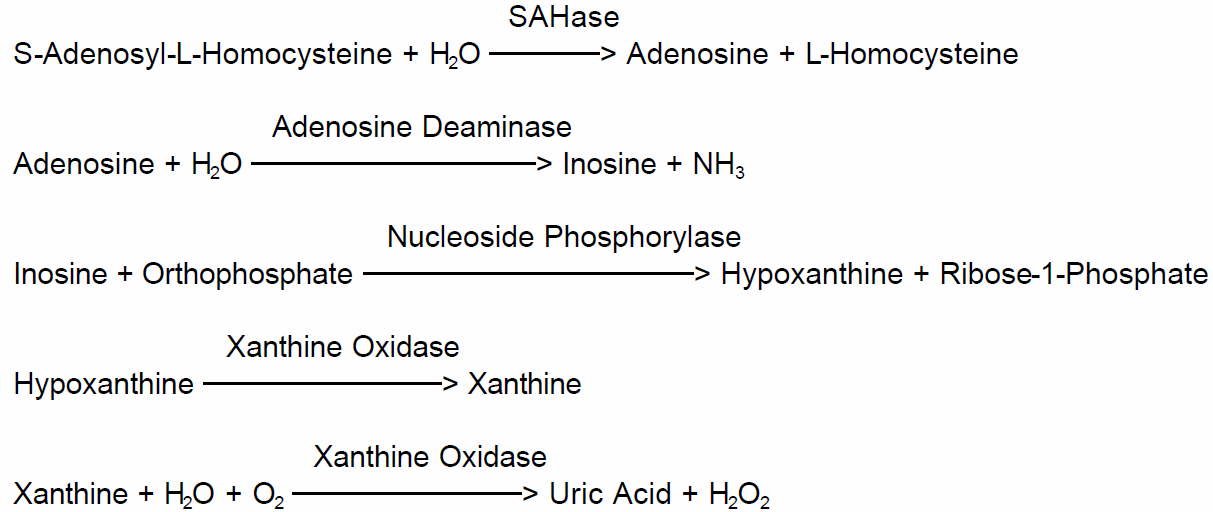
\includegraphics[width=\linewidth]{../idock/EnzymaticAssay.png}
\caption{Enzymatic assay of SAHH.}
\label{idock:EnzymaticAssay}
\end{figure}

\begin{table}
\centering
\begin{tabular}
{rcc}
\toprule
& Scitegic ECFP4 fingerprint & Daylight fingerprint\\
\midrule
HIV RT inhibitor & 1.00 & 1.00 \\
  SAHH inhibitor & 0.51 & 0.70 \\
   ADA inhibitor & 0.42 & 0.75 \\
   PNP inhibitor & 0.51 & 0.76 \\
\bottomrule
\end{tabular}
\caption{Tanimoto coefficients between TDF and the inhibitors of HIV RT, SAHH, ADA, and PNP.}
\label{idock:TanimotoCoefficients}
\end{table}

\subsection{Problem definition}

The problem is to discover a few promising compounds that inhibit HIV RT only, minimizing toxicity without affecting SAHH, ADA, or PNP. From the computational perspective, it is equivalent to shortlisting candidates from existing ligand databases such that they bind to HIV RT with a higher affinity and bind to SAHH, ADA, and PNP with a lower affinity. This can be done by protein-ligand docking.

\subsection{Proteins}

The crystal structures of HIV RT, SAHH, ADA, and PNP were collected from the Protein Data Bank (PDB) database \citep{539,537}. Protein-ligand complexes with PDB IDs of 2ZD1, 1LI4, 3IAR, and 3BGS were selected because they were crystallized at high resolutions (Table \ref{idock:SelectedPDBEntries}). Search spaces were then manually defined in cuboid shape to be large enough for ligands to freely translate and rotate inside.

\begin{table}
\centering
\begin{tabular*}
{\linewidth}
{@{\extracolsep{\fill}}ccccc}
\toprule
PDB ID & Protein & Ligand & Resolution & Box size (\AA\textsuperscript{3})\\
\midrule
2ZD1 & HIV RT & T27 & 1.80 \AA & 18 x 18 x 20\\
1LI4 & SAHH   & NAD & 2.01 \AA & 26 x 24 x 18\\
3IAR & ADA    & 3D1 & 1.52 \AA & 22 x 16 x 16\\
3BGS & PNP    & DIH & 2.10 \AA & 18 x 18 x 20\\
\bottomrule
\end{tabular*}
\caption{Selected PDB entries for HIV RT, SAHH, ADA, and PNP.}
\label{idock:SelectedPDBEntries}
\end{table}

\subsection{Ligands}

10,928 ligands were collected from the clean drug like subset of the ZINC database \citep{532}. These ligands satisfy Lipinski's \textit{Rule of Five} \citep{169} with the xLogP value of at most 5, the molecular weight between 150 Da and 500 Da, the number of hydrogen bond donors of at most 5, and the number of hydrogen bonds acceptors of at most 10.

\subsection{Experiments}

The experiments include 1) validation of Vina and idock to ensure they are suitable for docking ligands against the four proteins, and 2) comparison of their virtual screening performance in terms of execution time, memory usage, predicted free energy, and predicted conformations.

Vina x86 version 1.1.2 and idock x86\_64 version 1.0, the most recent versions of both programs at the moment these experiments were carried out, were used for experiments. Both programs were run on desktop computers with Intel Xeon Dual Quad Core 2.4GHz and 32GB RAM under Ubuntu 10.04.1 x86\_64. The CPUs support Intel's Hyper-Threading technology, so each computer consisting of 8 physical cores can execute up to 16 logical threads simultaneously.

\subsection{Program Validation}

The four crystal ligands extracted from the four PDB complexes were conformationally randomized and redocked against their proteins by Vina and idock. Figure \ref{idock:Redocking} shows the four proteins in complex with their corresponding crystal and docked ligands. The ligands rendered in green are the crystal ones, the ligands rendered in red are the ones docked by Vina, and the ligands rendered in blue are the ones docked by idock. Table \ref{idock:RMSD} shows the root mean square deviations (RMSDs) between the crystal and docked conformations. The RMSDs are all below 2.0 \AA, a publicly accepted positive control for correct bound structure prediction, indicating both programs are suitable for docking ligands against the four proteins. The RMSDs obtained by Vina are slightly better than those obtained by idock, especially for the case of PNP. This is probably due to the coarse estimation of $e_{intra}$ in idock, which does not form covalent bonds internally but simply relies on rotatable bonds to detect atom pair mobility.

\begin{figure}
\centering
\subfloat[HIV RT in complex with crystal and docked T27.]
{
  \label{subfig:2ZD1-T27}
  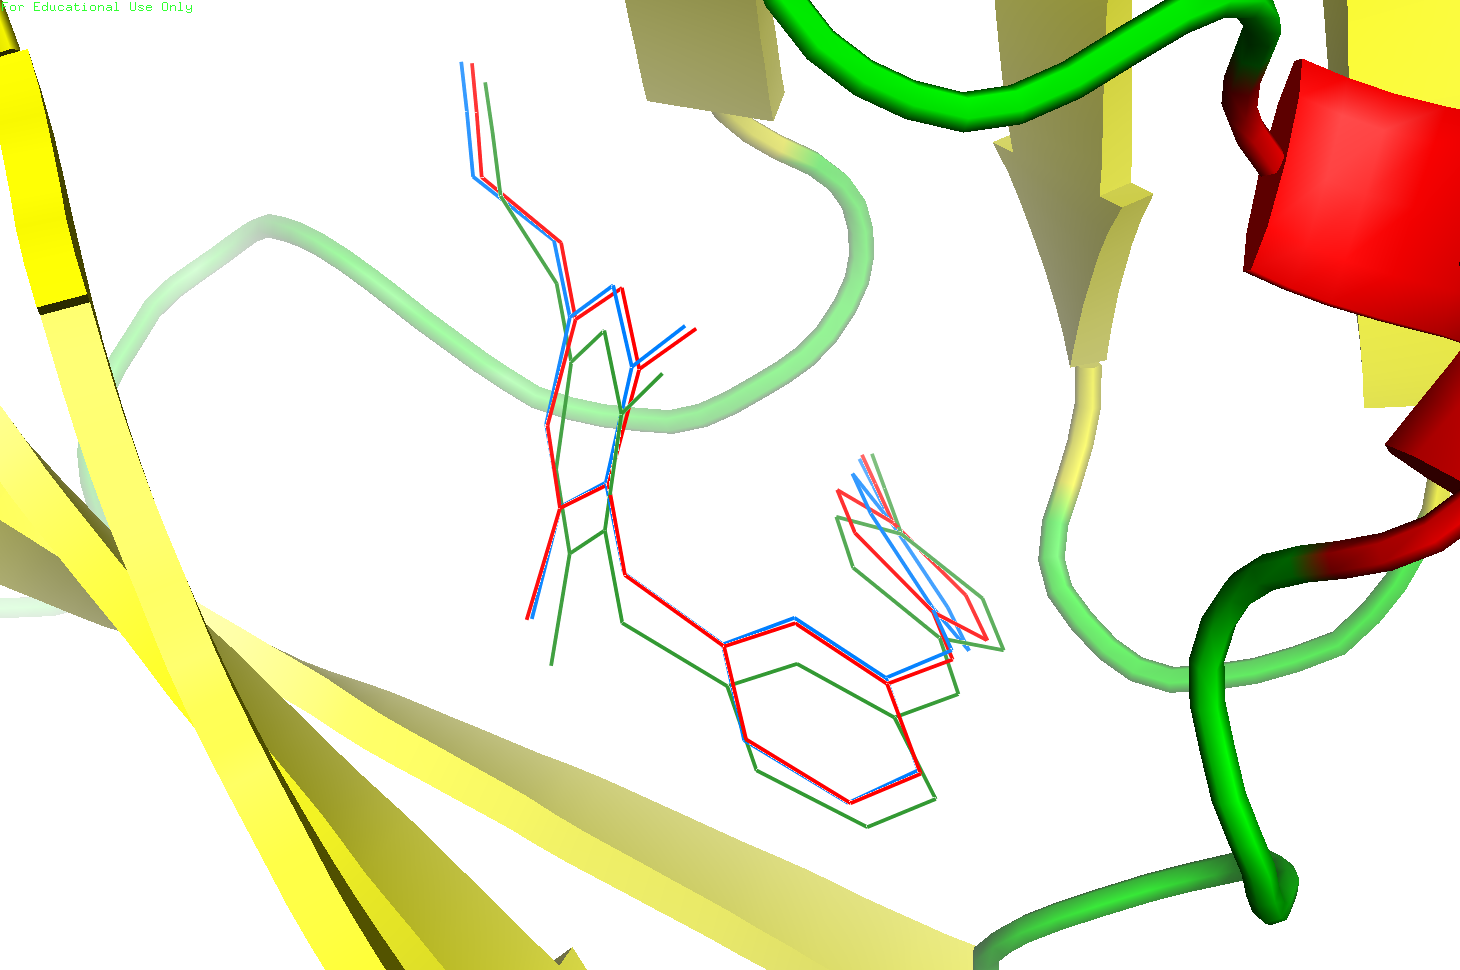
\includegraphics[width=0.236\linewidth]{../idock/2ZD1-T27.png}
}
\subfloat[SAHH in complex with crystal and docked NAD.]
{
  \label{subfig:1LI4-NAD}
  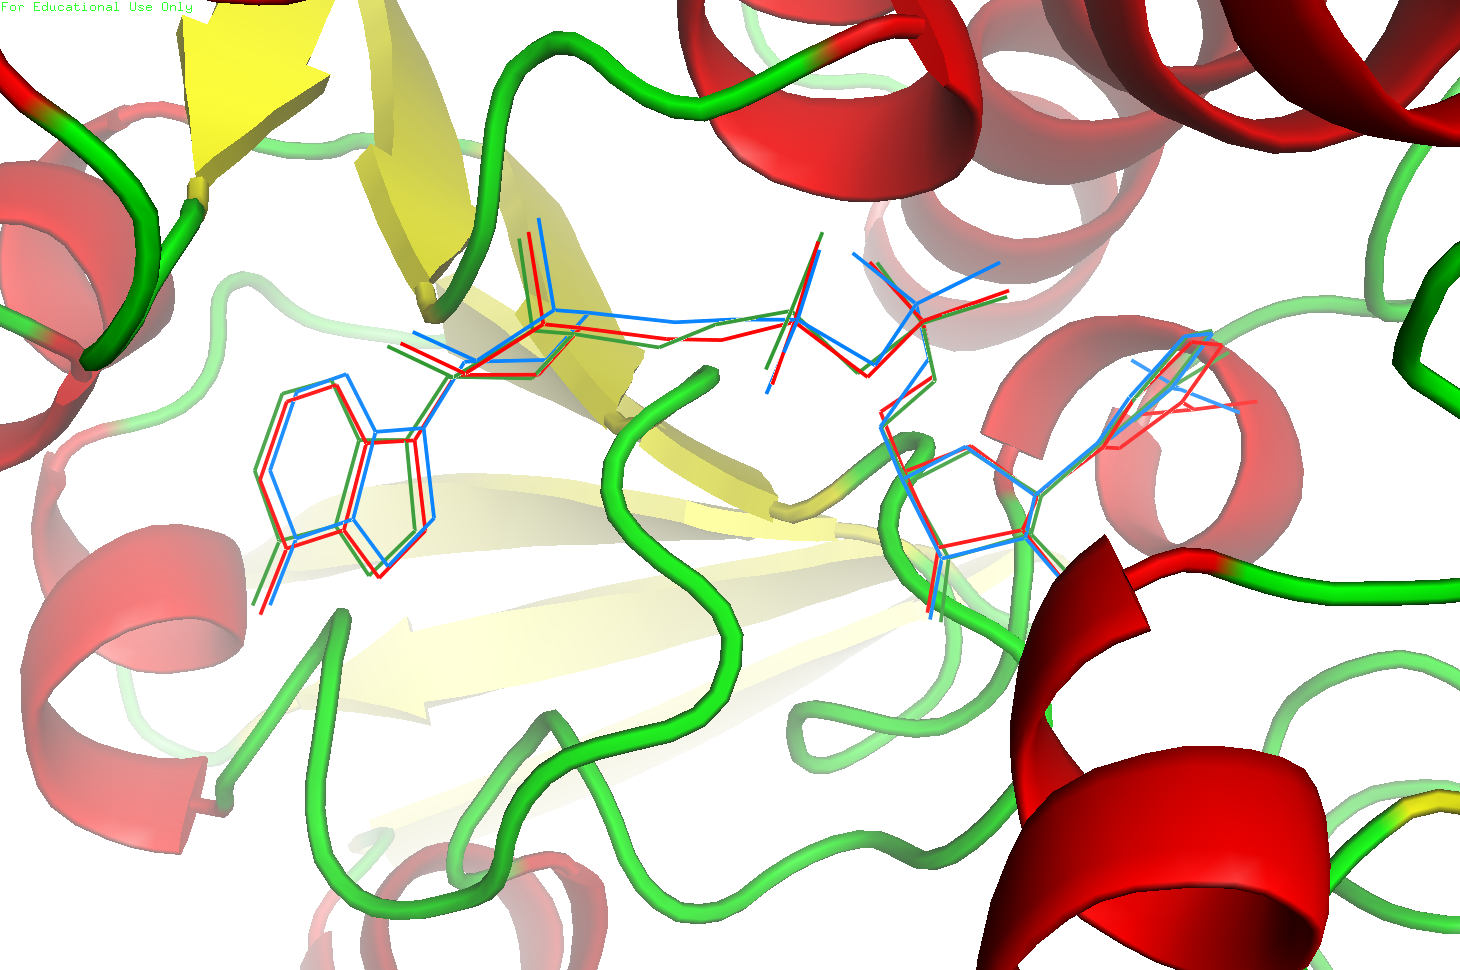
\includegraphics[width=0.236\linewidth]{../idock/1LI4-NAD.png}
}
\subfloat[ADA in complex with crystal and docked 3D1.]
{
  \label{subfig:3IAR-3D1}
  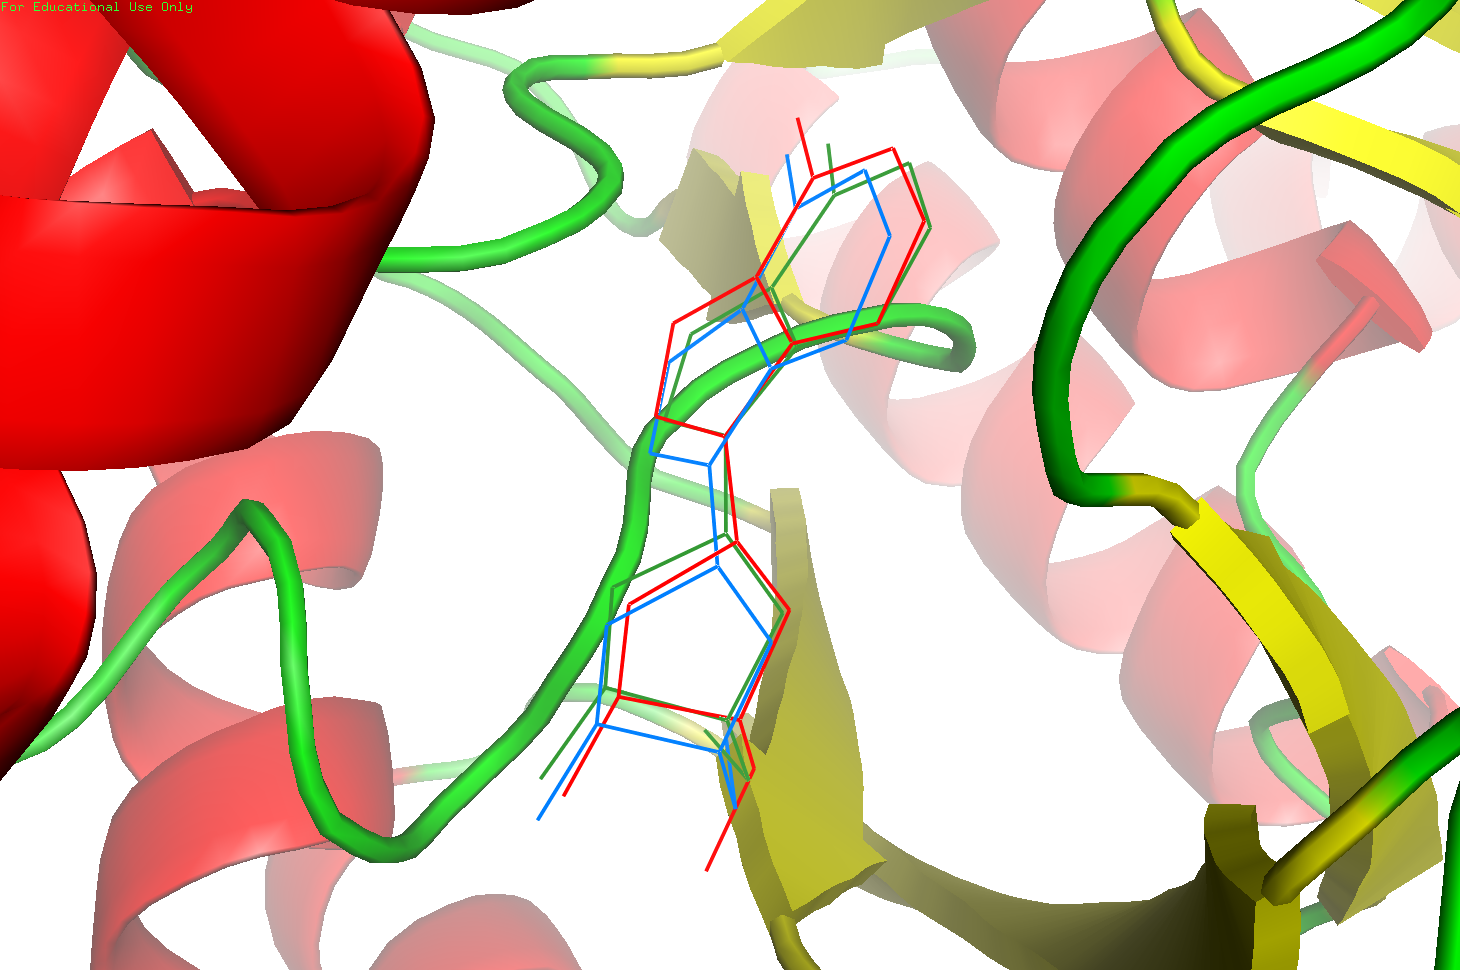
\includegraphics[width=0.236\linewidth]{../idock/3IAR-3D1.png}
}
\subfloat[PNP in complex with crystal and docked DIH.]
{
  \label{subfig:3BGS-DIH}
  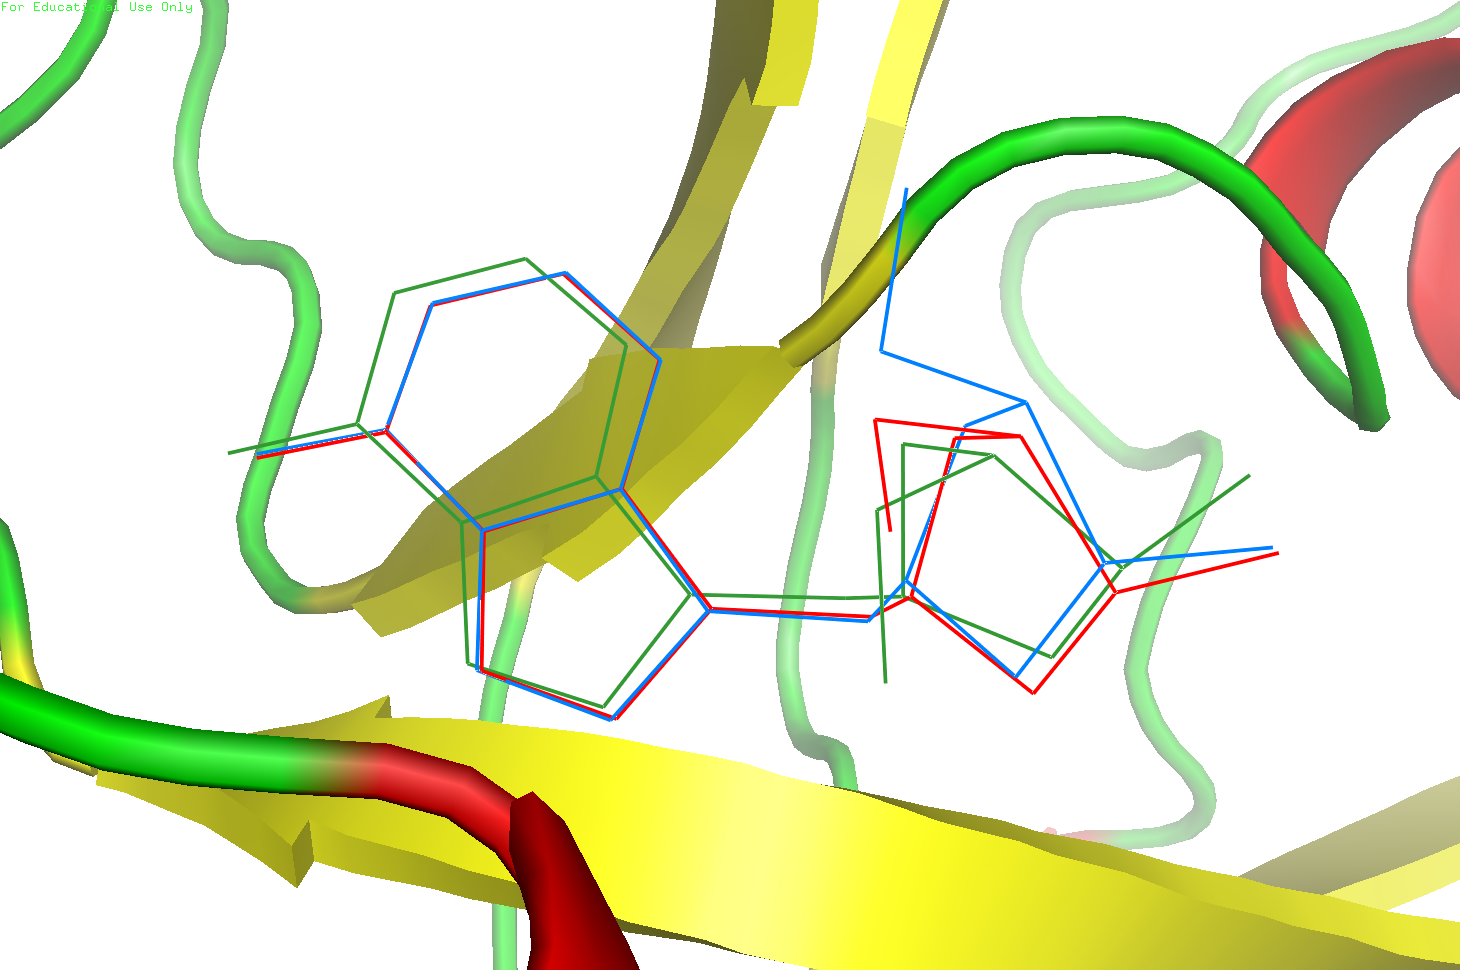
\includegraphics[width=0.236\linewidth]{../idock/3BGS-DIH.png}
}
\caption{HIV RT, SAHH, ADA, and PNP in complex with crystal and docked conformations of T27, NAD, 3D1, and DIH predicted by Vina and idock.}
\label{idock:Redocking}
\end{figure}

\begin{table}
\centering
\begin{tabular*}
{\linewidth}
{@{\extracolsep{\fill}}ccccc}
\toprule
PDB ID & Protein & Ligand & Vina (\AA) & idock (\AA)\\
\midrule
2ZD1 & HIV RT & T27 & 0.465 & 0.555\\
1LI4 & SAHH   & NAD & 0.537 & 0.593\\
3IAR & ADA    & 3D1 & 0.605 & 0.569\\
3BGS & PNP    & DIH & 0.756 & 1.170\\
\bottomrule
\end{tabular*}
\caption{RMSDs between the crystal and docked conformations of T27, NAD, 3D1, and DIH predicted by Vina and idock.}
\label{idock:RMSD}
\end{table}

\subsection{Virtual Screening}

Virtual screening was then carried out. 10,928 drug-like ligands were docked against the four proteins by Vina and idock. Since Vina can dock only one ligand in each run, a script containing 10,928 lines was generated and run instead, with each line being an execution of Vina to dock one individual ligand. Arguments to both programs were left as default. The GNU Time utility was used as profiler.

Table \ref{idock:ExecutionTimeAndMemoryUsage} compares the execution time and memory usage of docking 10,928 drug-like ligands against HIV RT, SAHH, ADA, and PNP by Vina and idock. Maximum CPU utilization is 1600\% due to Intel's Hyper-Threading technology. Vina required 428 to 504 CPU hours for one protein case, while idock required merely 88 to 184 CPU hours, resulting in a speedup of 2.5 to 4.8 and a screening performance of 1.3 drug-like ligands per CPU minute on average. In terms of elapsed time, the speedup was increased to as high as 6.3 to 10.4 because idock better utilized the CPU cores thanks to its efficient thread pool. idock also better utilized available memory to build grid maps at a high resolution and retained them along the way. Even though idock consumed more memory than Vina, its maximum resident set size did not exceed 1.5 GB, hence idock can be run on mainstream desktop computers.

\begin{table}
\centering
\begin{tabular*}
{\linewidth}
{@{\extracolsep{\fill}}rrrrr}
\toprule
Program & CPU Hours & Elapsed & CPU Util. & Max Mem Usage\\
\midrule
\multicolumn{5}{l}{\textbf{HIV RT}}\\
Vina  & 464 & 69:15:13 &  670\% & 126 MB\\
idock & 162 & 10:57:46 & 1474\% & 856 MB\\
Ratio & 2.9 &      6.3 & 0.45   & 0.15\\
\noalign{\smallskip\smallskip}
\multicolumn{5}{l}{\textbf{SAHH}}\\
Vina  & 460 & 78:53:59 &  582\% &   150 MB\\
idock & 184 & 12:24:24 & 1484\% & 1,368 MB\\
Ratio & 2.5 &      6.4 &  0.39  & 0.11\\
\noalign{\smallskip\smallskip}
\multicolumn{5}{l}{\textbf{ADA}}\\
Vina  & 504 & 74:22:37 &  677\% & 114 MB\\
idock & 127 &  8:46:12 & 1452\% & 764 MB\\
Ratio & 4.0 &      8.5 &  0.47  & 0.15\\
\noalign{\smallskip\smallskip}
\multicolumn{5}{l}{\textbf{PNP}}\\
Vina  & 428 & 62:19:55 &  687\% & 116 MB\\
idock &  88 &  5:58:19 & 1479\% & 857 MB\\
Ratio & 4.8 &     10.4 &  0.46  & 0.13\\
\noalign{\smallskip\smallskip}
\multicolumn{5}{l}{\textbf{Average}}\\
Vina  & 464 & 71:12:56 &  654\% & 124 MB\\
idock & 140 &  9:31:40 & 1472\% & 961 MB\\
Ratio & 3.3 &      7.5 & 0.44   & 0.13\\
\bottomrule
\end{tabular*}
\caption{Execution time and memory usage of docking 10,928 drug-like ligands by Vina and idock.}
\label{idock:ExecutionTimeAndMemoryUsage}
\end{table}

Table \ref{idock:RMSEAndRMSD} summarizes the root mean square errors (RMSEs) of free energies and RMSDs of conformations predicted by both programs. The RMSEs of free energies predicted by both programs vary from 0.31 to 0.46 kcal/mol, apparently less than 2.85 kcal/mol, the standard error obtained by Vina, indicating both programs predicted very similar free energies. For 27\% to 40\% of all the 10,928 ligands, the RMSD of the conformations predicted by both programs is equal to or less than 1.0 \AA, and for 49\% to 61\%, the RMSD is equal to or less than 2.0 \AA, indicating both programs predicted similar conformations for around half of the cases.

\begin{table}
\centering
\begin{tabular*}
{\linewidth}
{@{\extracolsep{\fill}}cccc}
\toprule
Protein & RMSE (kcal/mol) & Avg RMSD (\AA) & RMSD $\leq$ 2.0 \AA\\
\midrule
HIV RT & 0.35 & 2.554 & 61\%\\
SAHH   & 0.46 & 4.190 & 49\%\\
ADA    & 0.33 & 2.620 & 59\%\\
PNP    & 0.31 & 2.966 & 53\%\\
\bottomrule
\end{tabular*}
\caption{RMSEs of free energies and RMSDs of conformations predicted by Vina and idock.}
\label{idock:RMSEAndRMSD}
\end{table}

In order to shortlist a few promising ligands that bind to HIV RT with a high affinity but bind to SAHH, ADA, and PNP with a low affinity, filtering criteria were set. Ligands whose predicted free energies against HIV RT are below or equal to -11.0 kcal/mol and whose predicted free energies against the other three proteins are above or equal to -8.5 kcal/mol were shortlisted in Table \ref{idock:ShortlistedLigands}. The ZINC19888543 predicted by Vina and the ZINC44392991 predicted by idock were further investigated. Table \ref{idock:ZINC19888543-ZINC44392991} cites their predicted xLogP, number of hydrogen bond donors (HBD), number of hydrogen bond acceptors (HBA), molecular weight (MW), and number of rotatable bonds (NRB) from the ZINC database \citep{532}. Figures \ref{idock:Vina-ZINC19888543} and \ref{idock:idock-ZINC44392991}, rendered by PoseView 1.0.0 \citep{748}, show their predicted binding conformations in complex with the four proteins. Hydrogen bonds, salt bridges and metal interactions are highlighted as black dashed lines. Hydrophobic interactions are highlighted as green solid lines. Pi-Pi and Pi-cation interactions are highlighted as green dashed lines. It can be seen that ZINC19888543 interacts with HIV RT mainly through hydrophobic effects and Pi-Pi interactions, while ZINC44392991 interacts with HIV RT mainly through Pi-Pi interactions and hydrogen bonding.

\begin{table}
\centering
\begin{tabular*}
{\linewidth}
{@{\extracolsep{\fill}}ccccc}
\toprule
Ligand & HIV RT & SAHH & ADA & PNP\\
\midrule
\multicolumn{5}{l}{\textbf{Vina}}\\
ZINC04667184 & -11.1 & -6.6 & -7.5 & -7.5\\
ZINC06720921 & -11.0 & -7.4 & -8.0 & -8.4\\
ZINC14545253 & -11.0 & -6.5 & -8.0 & -7.6\\
ZINC19888543 & -11.1 & -7.9 & -7.8 & -7.8\\
ZINC26423182 & -11.1 & -6.4 & -7.8 & -7.4\\
ZINC49453017 & -11.3 & -7.1 & -8.3 & -7.6\\
ZINC60603133 & -11.0 & -7.9 & -8.3 & -7.4\\
\noalign{\smallskip\smallskip}
\multicolumn{5}{l}{\textbf{idock}}\\
ZINC03012460 & -11.3 & -8.3 & -7.8 & -7.3\\
ZINC04667184 & -11.2 & -7.6 & -7.7 & -8.0\\
ZINC44392991 & -11.1 & -7.7 & -7.3 & -8.1\\
ZINC49453017 & -11.6 & -7.3 & -8.3 & -7.8\\
\bottomrule
\end{tabular*}
\caption{Shortlisted ligands.}
\label{idock:ShortlistedLigands}
\end{table}

\begin{table}
\centering
\begin{tabular*}
{\linewidth}
{@{\extracolsep{\fill}}cccccc}
\toprule
Ligand & xLogP & HBD & HBA & MW (Da) & NRB\\
\midrule
ZINC19888543 & 4.48 & 1 & 3 & 342 & 3\\
ZINC44392991 & 4.24 & 1 & 6 & 391 & 6\\
\bottomrule
\end{tabular*}
\caption{Chemical properties of ZINC19888543 predicted by Vina and ZINC44392991 predicted by idock.}
\label{idock:ZINC19888543-ZINC44392991}
\end{table}

\begin{figure*}
\centering
\subfloat[HIV RT in complex with ZINC19888543.]
{
  \label{subfig:2ZD1-ZINC19888543}
  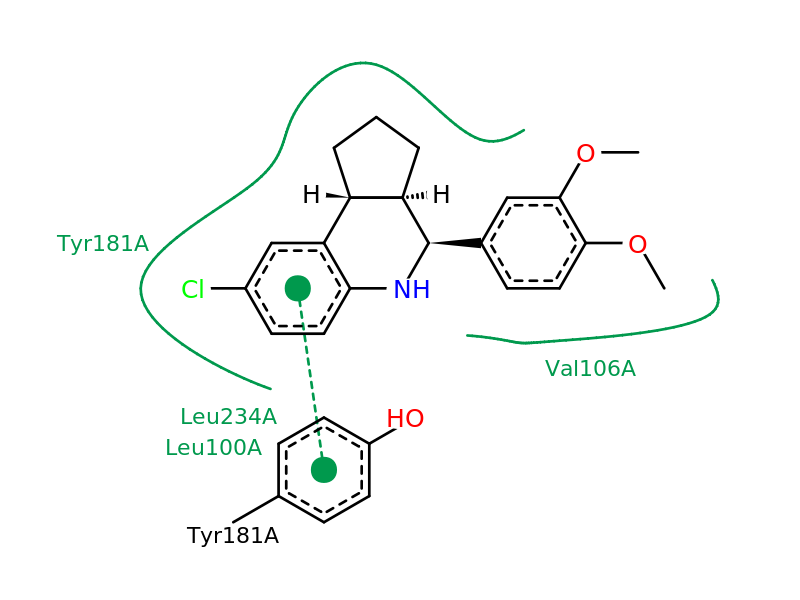
\includegraphics[width=0.236\linewidth]{../idock/2ZD1-ZINC19888543.png}
}
\subfloat[SAHH in complex with ZINC19888543.]
{
  \label{subfig:1LI4-ZINC19888543}
  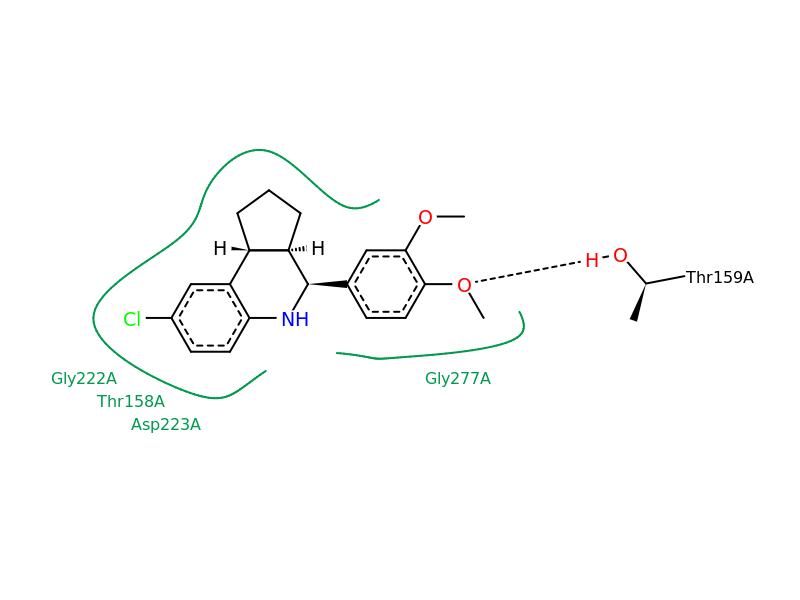
\includegraphics[width=0.236\linewidth]{../idock/1LI4-ZINC19888543.png}
}
\subfloat[ADA in complex with ZINC19888543.]
{
  \label{subfig:3IAR-ZINC19888543}
  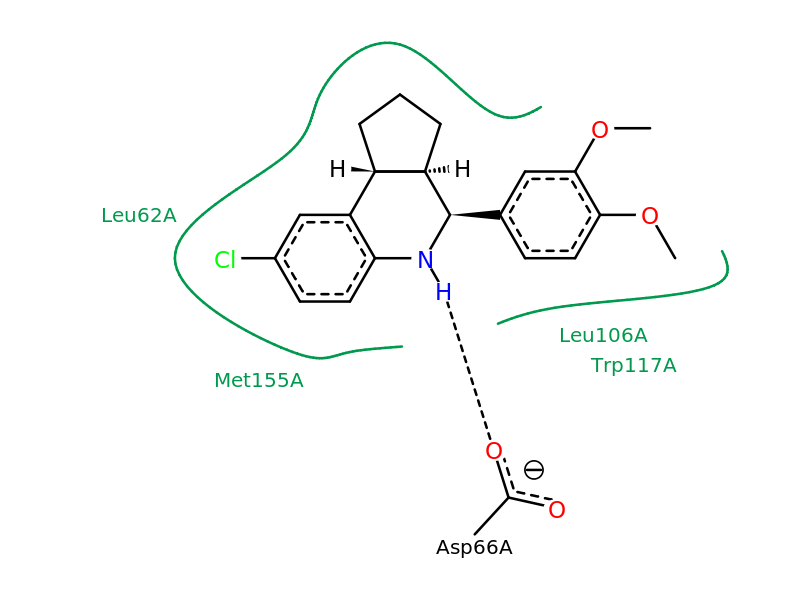
\includegraphics[width=0.236\linewidth]{../idock/3IAR-ZINC19888543.png}
}
\subfloat[PNP in complex with ZINC19888543.]
{
  \label{subfig:3BGS-ZINC19888543}
  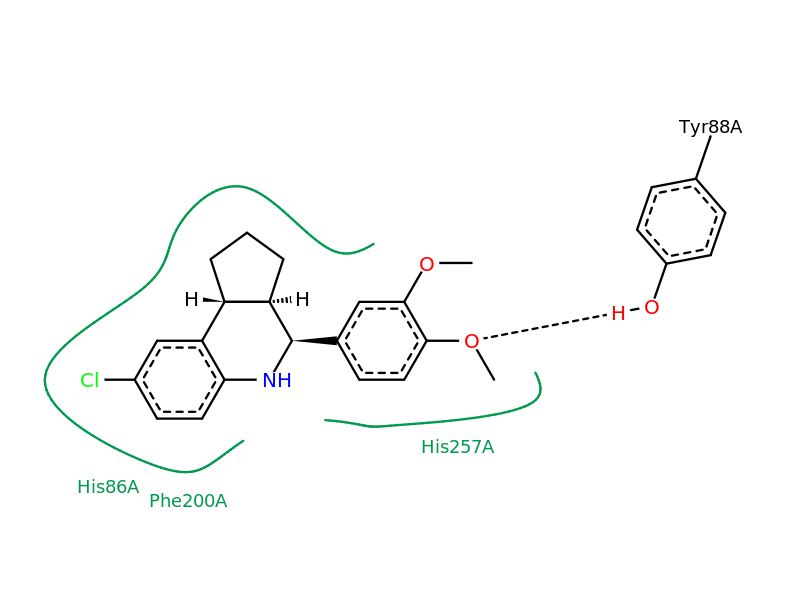
\includegraphics[width=0.236\linewidth]{../idock/3BGS-ZINC19888543.png}
}
\caption{HIV RT, SAHH, ADA, and PNP in complex with ZINC19888543 docked by Vina.}
\label{idock:Vina-ZINC19888543}
\end{figure*}

\begin{figure*}
\centering
\subfloat[HIV RT in complex with ZINC44392991.]
{
  \label{subfig:2ZD1-ZINC44392991}
  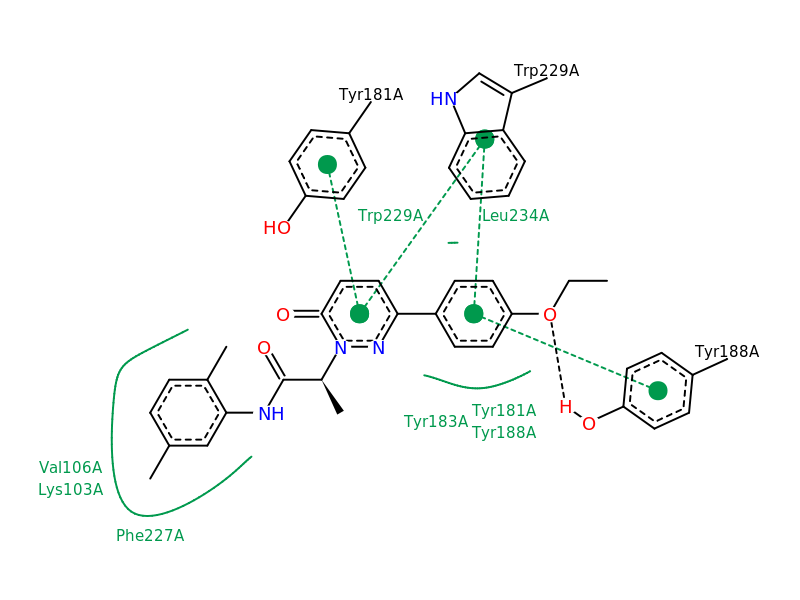
\includegraphics[width=0.236\linewidth]{../idock/2ZD1-ZINC44392991.png}
}
\subfloat[SAHH in complex with ZINC44392991.]
{
  \label{subfig:1LI4-ZINC44392991}
  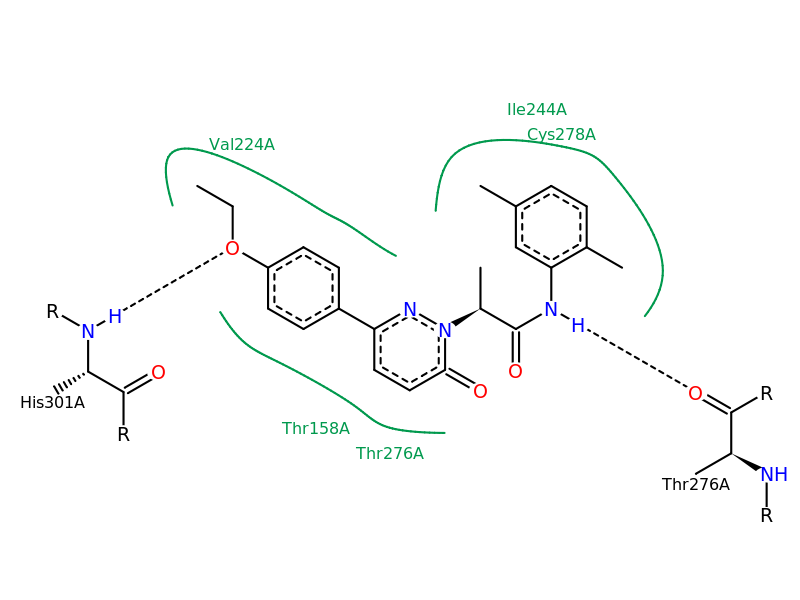
\includegraphics[width=0.236\linewidth]{../idock/1LI4-ZINC44392991.png}
}
\subfloat[ADA in complex with ZINC44392991.]
{
  \label{subfig:3IAR-ZINC44392991}
  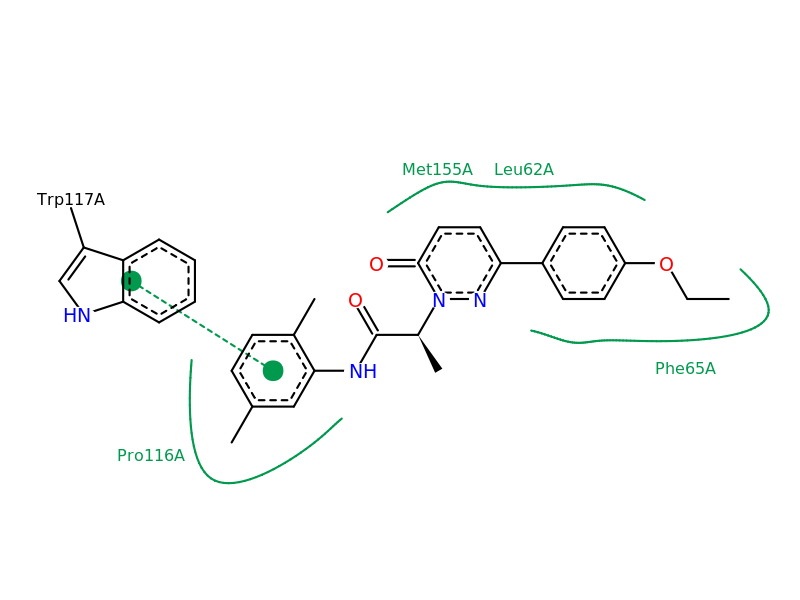
\includegraphics[width=0.236\linewidth]{../idock/3IAR-ZINC44392991.png}
}
\subfloat[PNP in complex with ZINC44392991.]
{
  \label{subfig:3BGS-ZINC44392991}
  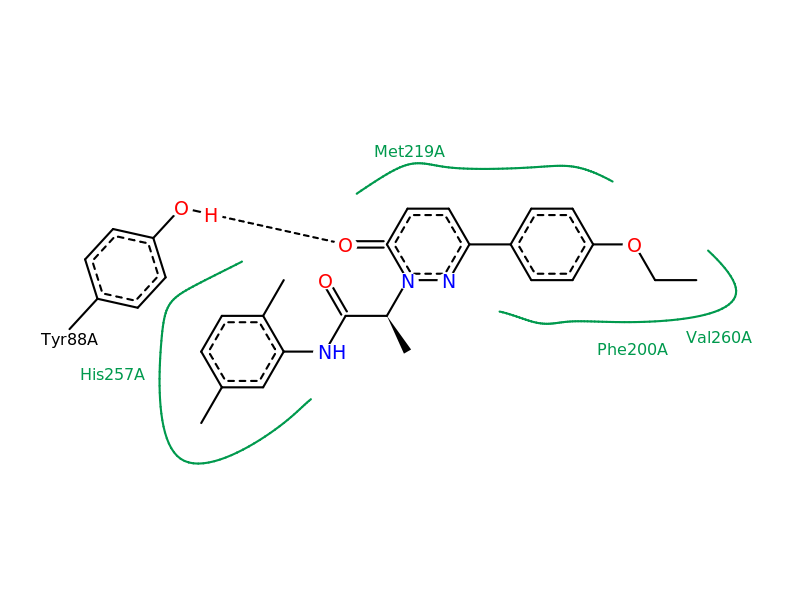
\includegraphics[width=0.236\linewidth]{../idock/3BGS-ZINC44392991.png}
}
\caption{HIV RT, SAHH, ADA, and PNP in complex with ZINC44392991 docked by idock.}
\label{idock:idock-ZINC44392991}
\end{figure*}

\section{Discussion}

Both Vina and idock adopt the same scoring function. They differ in their C++ implementations, data structures, numerical models, and Monte Carlo algorithms. idock implements its own thread pool to maintain a high CPU utilization throughout the entire screening procedure. It intensively utilizes modern C++11 techniques, particularly Rvalue references to avoid frequent reallocations of array data. It flattens Vina's tree-like recursive data structures into simple array structures to guarantee a high data cache hit rate. It automatically detects and deactivates inactive torsions and thus reduces the dimension of variables to optimize.

In Vina's official forum, there are tremendous requests for the support for virtual screening. The development of idock perfectly complements Vina. idock has built-in support for virtual screening. It searches for ligands in a user-specified folder and docks them one by one. It reuses threads and grid maps across multiple ligands. idock has very similar input and output arguments as Vina, so it should be quite easy for existing Vina users to transit to idock. Vina supports flexible receptor docking by rotating flexible side-chains. However, we have not yet implemented flexible receptor docking into idock at the moment, so users who need this kind of docking should refer to Vina.

\section{Conclusions}

We have developed idock, a multithreaded structure-based virtual screening tool for flexible ligand docking. It is capable of screening 1.3 drug-like ligands per CPU minute on average, making it a very competitive tool. Compared with Vina, idock achieves a speedup of 3.3 in terms of CPU time and a speedup of 7.5 in terms of elapsed time on average. But even so, it still required about 10 hours on average to dock 10,928 drug-like ligands against a certain protein, not to mention massive docking of millions of ligands. Virtual screening remains a time-consuming practice. Faster algorithms and implementations are highly desired. Porting idock to GPU using CUDA is one of our future directions.

We have developed idock for protein-ligand docking, inheriting from Vina the accurate scoring function and the efficient optimization algorithm, and meanwhile introducing a fruitful of innovations in C++ implementations, data structures, numerical models, and Monte Carlo algorithms. idock implements its own thread pool to maintain a high CPU utilization throughout the entire screening procedure. It intensively utilizes modern C++11 techniques, particularly Rvalue references to avoid frequent reallocations of array data. It flattens Vina's tree-like recursive data structures into simple array structures to guarantee a high data cache hit rate. It automatically detects and deactivates inactive torsions and thus reduces the dimension of variables to optimize.

In Vina's official forum, there are tremendous requests for the support for virtual screening. The development of idock perfectly complements Vina. idock has built-in support for virtual screening. It searches for ligands in a user-specified folder and docks them one by one. It reuses threads and grid maps across multiple ligands. idock has very similar input and output arguments as Vina, so it should be quite easy for existing Vina users to transit to idock. Vina supports flexible protein docking by rotating flexible side-chains. However, at the moment we have not yet implemented flexible protein docking, which has been proved helpful in some cases \citep{1084}, so users who need this kind of docking should refer to Vina.

We performed large-scale protein-ligand docking with idock, and noticed that the high-rank ligands were usually those comparatively rigid ligands with few active torsions. Such phenomenon can be explained by equation \eqref{idock:FlexibilityPenalty}. Fewer active torsions imply smaller denominator, or larger value in other words. We are considering replacing free energy by some ligand efficiency indexes \citep{335,336,337} for ranking.

\section{Availability}

idock 1.0 is free and open source under Apache License 2.0. Precompiled executables for 32-bit and 64-bit Linux, Windows, Mac OS X, FreeBSD and Solaris, 13 docking examples, and a doxygen file for generating API documentations are available at https://github.com/HongjianLi/idock.

\section{Future works}

The challenges of docking tools \citep{493}: protein flexibility, water molecules, metals. Another major factor that significantly limits the accuracy of today’s docking methods is protein flexibility upon ligand binding. The presence of water molecules critical to the binding of ligands adds another dimension to the docking problem.

The protein is assumed rigid in this study. \citep{1397} investigates the relationship between protein flexibility and binding free energy and present some useful hints for understanding when, and to what extent, flexibility should be considered.

Port idock to CUDA and OpenCL.
GASPRNG \citep{1401} GPU accelerated scalable parallel random number generator library using CUDA

The modern GPU (Graphics Processing Unit) has evolved from a fixed-function graphics pipeline to a programmable parallel processor with extremely high computational throughput and tremendous memory bandwidth at an affordable price. Performance evaluation of hybrid programming patterns for large CPU/GPU heterogeneous clusters has been carried out \citep{1035}. The past five years have seen a fruitful of algorithms for computer-aided drug discovery being ported to the GPU and gaining orders of magnitude of speedup over single threaded CPU counterparts. To name a few, such GPU-accelerated applications include FTMap \citep{722} for binding site mapping, CUDASW++2.0 \citep{189} for protein database search, the leader and the spread algorithms \citep{750} for compound selection, PIPER \citep{723}, PLANTS \citep{779}, parallelized AutoDock \citep{696}, GPUperTrAmber \citep{1270} and a transcription factor-DNA docking program \citep{1267,1266} for molecular docking, SIML \citep{726} and Tanimoto matrix calculation \citep{881} for chemical similarity calculation, OpenMM \citep{373}, MD-GPU \citep{374} and SPFP \citep{1261} for molecular dynamics, PAPER \citep{491} for molecular shape comparison, gWEGA \citep{1388} for molecular superposition and shape comparison, a k-centers algorithm for clustering conformations \citep{1275}, CAMPAIGN \citep{932} for data clustering, and visualization \citep{986}.

\chapterend
